%\documentclass[11pt]{article}
\documentclass{clv2}
\issue{?}{?}{2012}

%Document Head
\dochead{\date{}}

%\runningtitle{Learning Syntactic Categories Using Paradigmatic  Representations of Word Context}

\runningtitle{Unsupervised Part of Speech Induction}
\runningauthor{Mehmet Ali Yatbaz}

%\usepackage{acl2012}
\usepackage{times}
\usepackage{latexsym}
\usepackage{amsmath}
\usepackage{multirow}
\usepackage{url}
\usepackage{graphicx}
\usepackage{rotating}
\usepackage{pdflscape} %% more readable
\usepackage{caption}
% Table float box with bottom caption, box width adjusted to content
%\usepackage{lscape} %% less readable
%%% DY: Some consistency macros:

% many-to-one abbreviation
% 429 uses MTO
% Lamar uses M-to-1
% Maron uses MTO
% Lamar uses MTO
% Let us go with MTO
\newcommand{\mto}{\mbox{MTO}}
% Let us go with VM for V-measure
\newcommand{\vm}{\mbox{VM}}
% Adopt the .7654 convention rather than percentages like 76.54%.
% Define the results here for consistency
%% Spectral results
\newcommand{\spectralResult}{.5841}
\newcommand{\collapseResult}{.6882}
\newcommand{\spectralMtoPTB}{.5473}
\newcommand{\spectralVmPTB}{.4686}
\newcommand{\collapseMtoPTB}{.6834}
\newcommand{\collapseVmPTB}{.5087}
%% Scode resutls
\newcommand{\bgmto}{.7319 (.0088)}
\newcommand{\bgvm}{.6554 (.0039)}
\newcommand{\rpmto}{.7554 (.0055)}
\newcommand{\rpvm}{.6703 (.0037)}
\newcommand{\wsmto}{.7667 (.0056)} %type based one-tag restricted
\newcommand{\wsvm}{.6819 (.0029)} %type based one-tag restricted
\newcommand{\ftmto}{.8002 (.0070)} %type based + feature one-tag restricted
\newcommand{\ftvm}{.7163 (.0040)} %type based + feature one-tag restricted
\newcommand{\wsxymto}{.7030 (.0070)} %token based one-tag forced x+y
\newcommand{\wsxyvm}{.6006 (.0071)} %token based one-tag forced x+y
\newcommand{\wsymto}{.6366 (.0023)} %token based y
\newcommand{\wsyvm}{.4865 (.0051)} %token based y



\newcommand{\specialcell}[2][c]{%
  \begin{tabular}[#1]{@{}c@{}}#2\end{tabular}}

\title{Unsupervised Part of Speech Induction Using\\Paradigmatic Representations of Word Context}
\author{Mehmet Ali Yatbaz
\thanks{Artificial Intelligence Laboratory, Ko\c{c}
  University, 34450 Sar{\i}yer, \.Istanbul, Turkey. E-mail:
  myatbaz@ku.edu.tr, esert@ku.edu.tr, dyuret@ku.edu.tr}
}
\affil{Ko\c{c} University}

\author{Enis Sert}
\affil{Ko\c{c} University}
\author{Deniz Yuret}
\affil{Ko\c{c} University}

\begin{document}
\maketitle
%%

%Section 1
\section{Introduction}
\label{sec:intro}

Grammar rules apply not to individual words (e.g. dog, eat) but to
syntactic categories of words (e.g. noun, verb).  Thus constructing
syntactic categories (also known as lexical or part-of-speech
categories) is one of the fundamental problems in language
acquisition.

Linguists identify syntactic categories based on semantic, syntactic,
and morphological properties of words.  There is also evidence that
children use prosodic and phonological features to bootstrap syntactic
category acquisition \cite{ambridge2011child}.  However there is as
yet no satisfactory computational model that can match human
performance.  Thus identifying the best set of features and best
learning algorithms for syntactic category acquisition is still an
open problem.

Computational models of syntactic category acquisition in the
literature mainly rely on distributional analysis: Items that share
the same distribution (i.e. that occur in the same context) are
grouped into the same category.  The definition of ``the same
context'' vary across studies.  Algorithms based on the Hidden Markov
Model use class based n-grams to specify context
\cite{Brown:1992:CNG:176313.176316}, others use a frame of neighboring
words around the target word \cite{Schutze:1995:DPT:976973.976994}.
Our main contribution in this study is to introduce paradigmatic
features, i.e. features based on potential substitutes of the target
word, to represent word context.

Relationships between linguistic units can be classified into two
types: syntagmatic (concerning positioning), and paradigmatic
(concerning substitution).  Syntagmatic relations determine which
units can combine to create larger groups and paradigmatic relations
determine which units can be substituted for one another.
Figure~\ref{fig:paradigmatic} illustrates the paradigmatic vs
syntagmatic axes for words in a simple sentence and their possible
substitutes.

\begin{figure}[h] \centering
% Generated with LaTeXDraw 2.0.8
% Tue Jan 10 15:57:06 EET 2012
% \usepackage[usenames,dvipsnames]{pstricks}
% \usepackage{epsfig}
% \usepackage{pst-grad} % For gradients
% \usepackage{pst-plot} % For axes
\scalebox{1} % Change this value to rescale the drawing.
{
\begin{pspicture}(0,-1.6728125)(4.73474,1.6528125)
\usefont{T1}{ptm}{m}{n}
\rput(0.39520833,-0.6571875){\psframebox[linewidth=0.04]{the}}
\usefont{T1}{ptm}{m}{n}
\rput(1.8816146,-0.6571875){\psframebox[linewidth=0.04]{man}}
\usefont{T1}{ptm}{m}{n}
\rput(1.9886458,0.3428125){\psframebox[linewidth=0.04,linestyle=dashed,dash=0.16cm 0.16cm]{girl}}
\usefont{T1}{ptm}{m}{n}
\rput(3.3298957,-0.6571875){\psframebox[linewidth=0.04]{cried}}
\usefont{T1}{ptm}{m}{n}
\rput(3.2798958,0.3428125){\psframebox[linewidth=0.04,linestyle=dashed,dash=0.16cm 0.16cm]{died}}
\usefont{T1}{ptm}{m}{n}
\rput(3.3158333,1.3428125){\psframebox[linewidth=0.04,linestyle=dashed,dash=0.16cm 0.16cm]{sang}}
\usefont{T1}{pcr}{m}{n}
\rput(2.020677,-1.4671875){\footnotesize syntagmatic axis}
\usefont{T1}{pcr}{m}{n}
\rput{-90.0}(4.4150524,4.661927){\rput(4.507552,0.1328125){\footnotesize paradigmatic axis}}
\psline[linewidth=0.04cm,arrowsize=0.05291667cm 2.0,arrowlength=1.4,arrowinset=0.4]{<->}(0.13364583,-1.1671875)(3.9336457,-1.1671875)
\psline[linewidth=0.04cm,arrowsize=0.05291667cm 2.0,arrowlength=1.4,arrowinset=0.4]{<->}(4.133646,1.6328125)(4.133646,-1.1671875)
\psline[linewidth=0.04cm](0.81364584,-0.6671875)(1.4136459,-0.6671875)
\psline[linewidth=0.04cm](2.3936458,-0.6671875)(2.8136458,-0.6671875)
\psline[linewidth=0.04cm](1.9136459,0.0528125)(1.9136459,-0.4271875)
\psline[linewidth=0.04cm](3.3136458,0.0928125)(3.3136458,-0.3671875)
\psline[linewidth=0.04cm](3.3136458,1.0128125)(3.3136458,0.6328125)
\end{pspicture} 
}

\caption{Syntagmatic vs. paradigmatic axes for words in a simple
  sentence \cite{chandler2007semiotics}.}
\label{fig:paradigmatic}
\end{figure}

Both syntagmatic and paradigmatic relations of a word can be used to
represent its context.  In the syntagmatic case the context is
represented by a selection of neighboring words, in the paradigmatic
case it is represented by a set of possible substitutes.  In previous
studies of syntactic category learning the context representation has
been primarily syntagmatic, either implicit in the class based n-grams
of the standard Hidden Markov Model, or explicit in the construction
and clustering of left and right neighbors.

In this study we explore a paradigmatic representation of the context
of a word in syntactic category acquisition.  Specifically, the
context of a word is represented by a list of its possible substitutes
and their probabilities, which we call the {\em substitute vector}.
Note that the substitute vector is a function of the context only, not
the target word.  Thus in effect we are clustering contexts, not
words.  When word contexts are clustered based on their substitute
vectors they reveal a grouping that largely match the traditional part
of speech boundaries (\collapseResult\% many-to-one score using a
45-tag 24K word test corpus).
% standard HMM-EM gives 42\% on the same data.

Section~\ref{sec:related} gives a detailed review of related work.
The construction of the substitute vectors is described in
Section~\ref{sec:lm}.  To find out how to best make use of this new
paradigmatic representation, we explore different distance metrics
(Section~\ref{sec:dist}), dimensionality reduction methods
(Section~\ref{sec:dimreduce}), and clustering algorithms
(Section~\ref{sec:clustering}) for substitute vectors.  We note that
close to 95\% of the word occurrences in human labeled data are tagged
with their most frequent part of speech
\cite{Lee:2010:STU:1870658.1870741}, making one-tag-per-word a fairly
good first approximation.  Even ambicategory words generally have
fairly skewed part of speech distributions.
Section~\ref{sec:sparsity} looks at ways to increase the sparsity of
our solutions and demonstrates significant improvements using the
one-tag-per-word assumption and similarity metrics that introduce
sparsity.  Section~\ref{sec:discussion} discusses the results and
Section~\ref{sec:contrib} summarizes our contributions.



%Section 2
\section{Representing Word Context}
\label{sec:representation}

% example substitute vectors (both syntactic and semantic)

In this section we demonstrate the different contextual
representations in the part-of-speech induction (aka. syntactic word
categorization) literature and introduce the substitute words as an
alternative to the current context representations.  In the rest of
the paper the words in the vocabulary are referred as {\em types} and
the instances of types are referred as {\em tokens}.

The contextual representations can be categorized into three groups
based on the way they incorporate the local context information of the
target type or token: (1) syntagmatic representation, (2) Hidden
Markov Models (HMM) and (3) paradigmatic representation.  These
representations can be further subdivided into two subgroups based on
whether they group the types or the tokens.

%\subsection{Co-occurrences}
\paragraph{Syntagmatic Representation}

In syntagmatic representation the context is defined with the
neighboring words, typically co-occurrences with a single word on the
left or a single word on the right word called a ``frame'' (e.g., {\em
  {\bf the} dog {\bf is}; {\bf the} cat {\bf is}})
\cite{SchutzePe93,redington1998distributional,mintz2003frequent,20674613,lamar-EtAl:2010:Short,maron2010sphere}.
Turney and Pantel \shortcite{DBLP:journals/jair/TurneyP10} give a
broad overview of syntagmatic approaches and their applications within
the Vector Space Modeling framework.  Depending on the way they
incorporate co-occurences, these models can perform hard (type based)
or soft (token based) clustering.

Sch\"{u}tze \shortcite{SchutzePe93} represented the context of a word
type by concatenating its left and right co-occurence vectors.  These
vectors were calculated for each type by using the left and the right
neighbors of the type instances therefore they characterize the
distribution of the left and right neighboring tokens of the type.
One constraint of this representation is that it represents types
rather than tokens thus it is not possible to group the instances of
any type into the separate categories.

Mintz \shortcite{mintz2003frequent} showed on a subset of child
directed speech corpus (CHILDES) \cite{macwhinney2000childes} that
non-adjacent high frequent bigram frames are useful for the language
learners on the syntactic categorization of the tokens.  For example,
the tokens that are observed at ``\_'' in the frame ``{\em {\bf the}
  \_ {\bf is}}'' are assigned to the same category.  Using the top-45
frequent frames Mintz achieved an average of 98\% unsupervised
accuracy\footnote{Unsupervised accuracy was defined as the number of
  hits (when two intervening tokens that observed in the frame are
  from the same category) divided by number of false alarms (when two
  intervening tokens that observed in the frame are from different
  categories).}.  The main limitation of the top-45 frequent frames is
that they could only analyze the 6\% of the tokens on average due to
the sparsity.  Another drawback is that the tokens with only one
common neighbors could not exchange information.

St Clair et al.  \shortcite{20674613} extended the work of Mintz
\shortcite{mintz2003frequent} and introduced the flexible bigram
frames which represent the context by using the left and the right
bigrams separately.  As a result tokens with a common left or right
bigram can exchange information and might be grouped together.  For
instance, two tokens that are observed at ```\_'' in ``{\em {\bf the}
  \_ {\bf is}}'' and ``{\em {\bf a} \_ {\bf is}}'' can be categorized
together due to the shared right bigram ``{\em{\bf is}}''.  Using a
feed forward connectionist model they showed that the flexible frames
are statistically better than the frequent frames in terms of the
supervised accuracy\footnote{In order to perform meaningful
  comparisons they used all the frequent frames instead of the top-45
  ones.}.  They also showed that representing token contexts only with
the left or the right bigram is statistically better than the frequent
frames but worse than the flexible frames in terms of supervised
accuracy.  Both Mintz \shortcite{mintz2003frequent} and St Clair
\shortcite{20674613} did not report any results with contexts larger
than bigram since as the context is enriched, the re-occurrence
frequency of a frame becomes lower which causes the data sparsity
\cite{manning99foundations}.

%\subsection{HMM}
\paragraph{HMM} 
Prototypical HMM uses a bigram structure where tokens are generated by
latent categories and learns the latent category sequence that
generates the given word sequence instead of clustering tokens
directly
\cite{Brown:1992:CNG:176313.176316,blunsom-cohn:2011:ACL-HLT2011,goldwater-griffiths:2007:ACLMain,johnson:2007:EMNLP-CoNLL2007,Ganchev:2010:PRS:1859890.1859918,bergkirkpatrick-klein:2010:ACL,Lee:2010:STU:1870658.1870741}.
The POS induction literature focused on the first and second order
HMMs since the higher order HMMs have additional complicating
factors\footnote{The number of parameters in a prototypical HMM
  quadratically increases as the HMM order increases.}  and require
more complex training procedures \cite{johnson:2007:EMNLP-CoNLL2007}.
Depending on the design and the training procedure HMM models can
group types or tokens which are detailed in Section \ref{sec:related}.

%\subsection{Substitute words}
\paragraph{Paradigmatic Representation} 

In the paradigmatic representation context is defined as the
distribution of the substitute words in that context.  Sch\"{u}tze
\shortcite{Schutze:1995:DPT:976973.976994} incorporates paradigmatic
information by concatenating the left co-occurrence and the right
co-occurrence vectors of the right and the left tokens, respectively
and grouped the tokens that have similar vectors.  The vectors from
the neighbors include potential substitutes.  Yatbaz et
al. \shortcite{yatbaz-sert-yuret:2012:EMNLP-CoNLL} calculate the most
likely substitute words of a word in a given context and clusters the
types that have similar substitutes.

Our paradigmatic representation is related to the second order
co-occurrences used in \cite{Schutze:1995:DPT:976973.976994}.  Our
method improves on his foundation from three aspects: (1) it can
cluster both the types and tokens (2) it uses a 4-gram language model
rather than bigram statistics, (3) it includes the whole 78,498 word
vocabulary rather than the most frequent 250 words.  More importantly,
rather than simply concatenating the vectors that represent the target
word with vectors that represent the context we use a co-occurrence
modeling algorithm.

Similarly, Sch{\"u}tze and Pedersen \shortcite{SchutzePe93} define the
words that frequently co-occur together as the {\em syntagmatic
  associates} and words that have similar left and right neighbors as
the {\em paradigmatic parallels}.  We find that representing the
paradigmatic axis more directly using substitute vectors rather than
frequent neighbors improves part of speech induction.

Sahlgren \shortcite{sahlgren2006word} gives a detailed analysis of
paradigmatic and syntagmatic relations in the context of word-space
models used to represent the word meanings.  Sahlgren's paradigmatic
model represents word types using co-occurrence counts of their
frequent neighbors, in contrast to his syntagmatic model that
represents word types using counts of contexts (documents, sentences)
they occur in.  Our substitute vectors do not represent word types at
all, but {\em contexts of word tokens} using probabilities of likely
substitutes.  Sahlgren finds that in word-spaces built by frequent
neighbor vectors, more nearest neighbors share the same part of speech
compared to word-spaces built by context vectors.

The two examples below illustrate the advantages of paradigmatic
representation in uncovering similarities where no overt similarity
that can be captured by a syntagmatic representation exists.  The word
``director'' from the first sentence and the word ``chief'' from the
second one have no common neighbors in their 4-gram neighborhood.  The
paradigmatic representation captures the similarity of these words by
suggesting the same top substitutes for both (the numbers in
parentheses give substitute probabilities):
\begin{quote}
  (1) \noindent{\em ``Pierre Vinken, 61 years old, will join the board as a nonexecutive {\bf director} Nov.~29.''}\\
% {\bf the:} its (.9011), the (.0981), a (.0006), $\ldots$\\
  \noindent{\bf director:} chairman (.8242), director (.0127),
  directors (.0127) $\ldots$
\end{quote}

\begin{quote}
  % (2) \noindent {\em ``Blacks and Hispanics currently make up 38 \% of the city 's population and hold only 25 \% of the seats on the {\bf council} .''}\\
  % (2) \noindent {\em ``$\ldots$ and hold only 25 \% of the seats on the {\bf council} .''}\\
% \noindent {\bf council:} board (.6591), company (.0795), firm (.0542), bank (.0154), $\ldots$
  (2) \noindent {\em ``$\ldots$ Joseph Corr was succeeded by Frank Lorenzo , {\bf chief} of parent Texas Air .''}\\
  \noindent {\bf chief:} chairman (.09945), president (.0031),
  directors (.0012) $\ldots$
\end{quote}

The high probability substitutes reflect both semantic and syntactic
properties of the context.  Top substitutes for ``director'' and
``chief'' are not only nouns, but specifically nouns compatible with
the semantic context.  Top substitutes for the word ``the'' in the
first example consist of words that can act as determiners: its
(.9011), the (.0981), a (.0006), $\ldots$.

%% \subsection{Substitute Vectors}
%% \label{sec:subthr}
%% %%substitute vector applications

%% In this section we explore the usage of substitute vectors within the
%% context clustering framework by comparing similarity metrics,
%% dimensionality reduction techniques and clustering methods.  The first
%% subsection describes the computation of substitute vectors using a
%% statistical language model.  Section~\ref{sec:dist} gives a detailed
%% comparison of similarity metrics in the high dimensional substitute
%% vector space.  Section~\ref{sec:dimreduce} analyzes the application of
%% dimensionality reduction algorithms to substitute vectors.
%% Section~\ref{sec:clustering} presents a comparison of clustering
%% methods on the PTB.

%% \subsection{Computation of Substitute Vectors}
%% \label{sec:subcomp}

%% In this study, we predict the syntactic category of a word in a given
%% context based on its substitute vector.  The dimensions of the
%% substitute vector represent words in the vocabulary, and the entries
%% in the substitute vector represent the probability of those words
%% being used in the given context.  Note that the substitute vector is a
%% function of the context only and is indifferent to the target word.

%% %This section details the choice of the data set, the vocabulary and
%% %the estimation of substitute vector probabilities.

%% %% % what is the test data
%% %% The Wall Street Journal Section of the Penn Treebank \cite{treebank3}
%% %% was used as the test corpus (1,173,766 tokens, 49,206 types).
%% %% % what is the tag set
%% %% The treebank uses 45 part of speech tags which is the set we used as
%% %% the gold standard for comparison in our experiments.
%% %% % what is the LM training data
%% %% %Train => 5181717 126019973 690121813
%% %% To compute substitute probabilities we trained a language model using
%% %% approximately 126 million tokens of Wall Street Journal data
%% %% (1987-1994) extracted from CSR-III Text \cite{csr3text} (we excluded
%% %% the test corpus).
%% %% % how is the language model trained
%% %% We used SRILM \cite{Stolcke2002} to build a 4-gram language model with
%% %% Kneser-Ney discounting.
%% %% % what is the vocabulary
%% %% Words that were observed less than 20 times in the language model
%% %% training data were replaced by \textsc{unk} tags, which gave us a
%% %% vocabulary size of 78,498.
%% %% % perplexity
%% %% The perplexity of the 4-gram language model on the test corpus is 96.

%% % how are the substitutes computed
%% It is best to use both the left and the right context when estimating the
%% probabilities for potential lexical substitutes.  For example, in
%% \emph{``He lived in San Francisco suburbs.''}, the token \emph{San}
%% would be difficult to guess from the left context but it is almost
%% certain looking at the right context.  We define $c_w$ as the $2n-1$
%% word window centered around the target word position: $w_{-n+1} \ldots
%% w_0 \ldots w_{n-1}$ ($n=4$ is the n-gram order).  The probability of a
%% substitute word $w$ in a given context $c_w$ can be estimated as:
%% \begin{eqnarray}
%%   \label{eq:lm1}P(w_0 = w | c_w) & \propto & P(w_{-n+1}\ldots w_0\ldots w_{n-1})\\
%%   \label{eq:lm2}& = & P(w_{-n+1})P(w_{-n+2}|w_{-n+1})\nonumber\\
%%   &&\ldots P(w_{n-1}|w_{-n+1}^{n-2})\\
%%   \label{eq:lm3}& \approx & P(w_0| w_{-n+1}^{-1})P(w_{1}|w_{-n+2}^0)\nonumber\\
%%   &&\ldots P(w_{n-1}|w_0^{n-2})
%% \end{eqnarray}
%% where $w_i^j$ represents the sequence of words $w_i w_{i+1} \ldots
%% w_{j}$.  In Equation \ref{eq:lm1}, $P(w|c_w)$ is proportional to
%% $P(w_{-n+1}\ldots w_0 \ldots w_{n-1})$ because the words of the
%% context are fixed.  Terms without $w_0$ are identical for each
%% substitute in Equation \ref{eq:lm2} therefore they have been dropped
%% in Equation \ref{eq:lm3}.  Finally, because of the Markov property of
%% n-gram language model, only the closest $n-1$ words are used in the
%% experiments.

%% Near the sentence boundaries the appropriate terms were truncated in
%% Equation \ref{eq:lm3}.  Specifically, at the beginning of the sentence
%% shorter n-gram contexts were used and at the end of the sentence terms
%% beyond the end-of-sentence token were dropped.  

%% Rest of this section details the choice of the data set, the
%% vocabulary and the estimation of substitute probabilities.
%% For computational efficiency only the top 100 substitutes and their
%% unnormalized probabilities were computed for each of the 1,173,766
%% positions in the test set\footnote{The substitutes with unnormalized
%%   log probabilities can be downloaded from
%%   \mbox{\url{http://goo.gl/jzKH0}}.  For a description of the {\sc
%%     fastsubs} algorithm used to generate the substitutes please see
%%   \mbox{\url{http://arxiv.org/abs/1205.5407v1}}.  {\sc fastsubs}
%%   accomplishes this task in about 5 hours, a naive algorithm that
%%   looks at the whole vocabulary would take more than 6 days on a
%%   typical 2012 workstation.}.  The probability vectors for each
%% position were normalized to add up to 1.0 giving us the final
%% substitute vectors used in the rest of this study.

%% % what is the test data
%% The Wall Street Journal Section of the Penn Treebank (PTB) \cite{treebank3}
%% was used as the test corpus (1,173,766 tokens, 49,206 types) to be
%% induced.
%% % what is the tag set
%% The treebank uses 45 part-of-speech tags which is the set we used as
%% the gold standard for comparison in our experiments.
%% % what is the LM training data
%% %Train => 5181717 126019973 690121813
%% To compute substitute probabilities we trained a language model using
%% approximately 126 million tokens of Wall Street Journal data
%% (1987-1994) extracted from CSR-III Text \cite{csr3text} (excluding
%% sections of the PTB).
%% % how is the language model trained
%% We used SRILM \cite{Stolcke2002} to build a 4-gram language model with
%% Kneser-Ney discounting.
%% % what is the vocabulary
%% Words that were observed less than 20 times in the language model
%% training data were replaced by \textsc{unk} tags, which gave us a
%% vocabulary size of 78,498.
%% % what is the test data
%% % perplexity
%% The perplexity of the 4-gram language model on the test corpus is 96.

%Section 3
%%%


%% % Section 3, 3.1
%% \section{Substitute Theory and Application}
\label{sec:subthr}
%%substitute vector applications

Substitute theory is a special case of Vector Space Models (VSM)
\cite{DBLP:journals/jair/TurneyP10} in which meaning of a word is
represented by high dimensional substitute vectors.  Substitute
vectors capture the word--context relation by constructing probability
vectors therefore context of each word is represented by its possible
substitutes instead of the neighboring words.  One problem of VSM is
that vectors do not keep the information of identity, ortographic or
morphological features of words and there is no standard way of
incorporating these extra features into VSM.  Thus instead of
focusing on how to incorporate extra features to the vectors, we
dedicate this section to determine the best usage of substitute
vectors within the VSM framework by comparing similarity metrics
together with dimension reduction and clustering methods on UPOS
without using the word identities or any other features.

%% Following Turney and Pantel \shortcite{DBLP:journals/jair/TurneyP10}
%% we determine the best usage of substitute vectors by comparing various
%% well knwon similarity metrics together with dimensionality reduction
%% and clustering algorithms.

%% [??Vector space model paper distance, dim red, matrix type.]

%% To determine the best usage scenerio of high dimensional substitute
%% vectors in terms of both \mto accuracies and computational
%% performance.

%% we compare well known distance metrics to distinguish best similarity
%% measure between the vectors.  We also apply dimensionality reduction
%% algorithms to reduce the computaional complexy.

In the following section, we describe the theory and computation of
substitute vectors using a statistical language model.
Section~\ref{sec:dist} gives a detailed comparison of similarity
metrics in high dimensional substitute vector space.
Section~\ref{sec:dimreduce} analyzes application of possible
dimensionality reduction algorithms to our problem.
Section~\ref{sec:clustering} presents comparison of various clustering
techniques and applies the findings of the previous sections to the
PTB.

In section~\ref{sec:code} we discuss the co-occurrence modeling as an
alternative to VSM.

\subsection{Computation of Substitute Vectors}
\label{sec:subcomp}

In this study, we predict the syntactic category of a word in a given
context based on its substitute vector.  The dimensions of the
substitute vector represent words in the vocabulary, and the entries
in the substitute vector represent the probability of those words
being used in the given context.  Note that the substitute vector is a
function of the context only and is indifferent to the target word.

%This section details the choice of the data set, the vocabulary and
%the estimation of substitute vector probabilities.

%% % what is the test data
%% The Wall Street Journal Section of the Penn Treebank \cite{treebank3}
%% was used as the test corpus (1,173,766 tokens, 49,206 types).
%% % what is the tag set
%% The treebank uses 45 part-of-speech tags which is the set we used as
%% the gold standard for comparison in our experiments.
%% % what is the LM training data
%% %Train => 5181717 126019973 690121813
%% To compute substitute probabilities we trained a language model using
%% approximately 126 million tokens of Wall Street Journal data
%% (1987-1994) extracted from CSR-III Text \cite{csr3text} (we excluded
%% the test corpus).
%% % how is the language model trained
%% We used SRILM \cite{Stolcke2002} to build a 4-gram language model with
%% Kneser-Ney discounting.
%% % what is the vocabulary
%% Words that were observed less than 20 times in the language model
%% training data were replaced by \textsc{unk} tags, which gave us a
%% vocabulary size of 78,498.
%% % perplexity
%% The perplexity of the 4-gram language model on the test corpus is 96.

% how are the substitutes computed
It is best to use both left and right context when estimating the
probabilities for potential lexical substitutes.  For example, in
\emph{``He lived in San Francisco suburbs.''}, the token \emph{San}
would be difficult to guess from the left context but it is almost
certain looking at the right context.  We define $c_w$ as the $2n-1$
word window centered around the target word position: $w_{-n+1} \ldots
w_0 \ldots w_{n-1}$ ($n=4$ is the n-gram order).  The probability of a
substitute word $w$ in a given context $c_w$ can be estimated as:
\begin{eqnarray}
  \label{eq:lm1}P(w_0 = w | c_w) & \propto & P(w_{-n+1}\ldots w_0\ldots w_{n-1})\\
  \label{eq:lm2}& = & P(w_{-n+1})P(w_{-n+2}|w_{-n+1})\nonumber\\
  &&\ldots P(w_{n-1}|w_{-n+1}^{n-2})\\
  \label{eq:lm3}& \approx & P(w_0| w_{-n+1}^{-1})P(w_{1}|w_{-n+2}^0)\nonumber\\
  &&\ldots P(w_{n-1}|w_0^{n-2})
\end{eqnarray}
where $w_i^j$ represents the sequence of words $w_i w_{i+1} \ldots
w_{j}$.  In Equation \ref{eq:lm1}, $P(w|c_w)$ is proportional to
$P(w_{-n+1}\ldots w_0 \ldots w_{n+1})$ because the words of the
context are fixed.  Terms without $w_0$ are identical for each
substitute in Equation \ref{eq:lm2} therefore they have been dropped
in Equation \ref{eq:lm3}.  Finally, because of the Markov property of
n-gram language model, only the closest $n-1$ words are used in the
experiments.

Near the sentence boundaries the appropriate terms were truncated in
Equation \ref{eq:lm3}.  Specifically, at the beginning of the sentence
shorter n-gram contexts were used and at the end of the sentence terms
beyond the end-of-sentence token were dropped.  Rest of this section
details the choice of the data set, the vocabulary and the estimation
of substitute probabilities.

%% For computational efficiency only the top 100 substitutes and their
%% unnormalized probabilities were computed for each of the 1,173,766
%% positions in the test set\footnote{The substitutes with unnormalized
%%   log probabilities can be downloaded from
%%   \mbox{\url{http://goo.gl/jzKH0}}.  For a description of the {\sc
%%     fastsubs} algorithm used to generate the substitutes please see
%%   \mbox{\url{http://arxiv.org/abs/1205.5407v1}}.  {\sc fastsubs}
%%   accomplishes this task in about 5 hours, a naive algorithm that
%%   looks at the whole vocabulary would take more than 6 days on a
%%   typical 2012 workstation.}.  The probability vectors for each
%% position were normalized to add up to 1.0 giving us the final
%% substitute vectors used in the rest of this study.

% what is the LM training data
%Train => 5181717 126019973 690121813

To compute substitute probabilities we trained a language model using
approximately 126 million tokens of Wall Street Journal data
(1987-1994) extracted from CSR-III Text \cite{csr3text} (excluding
sections of the PTB).
% how is the language model trained
We used SRILM \cite{Stolcke2002} to build a 4-gram language model with
Kneser-Ney discounting.
% what is the vocabulary
Words that were observed less than 500 times in the LM training data
were replaced by \textsc{unk} tags, which gave us a vocabulary size of
12,672.
% what is the test data
The first 24,020 tokens of the Penn Treebank Wall Street Journal
Section 00 (PTB24K) was used as the test corpus to be induced.  Corpus
size kept small in order to efficiently compute full distance
matrices.  Substitution probabilities for 12,672 vocabulary words were
computed at each of the 24,020 positions.
% perplexity
The perplexity of the 4-gram language model on the test corpus was
55.4 which is quite low due to using a small 
vocabulary and in-domain data.
% what is the tag set
The treebank uses 45 part-of-speech tags which is the set we used as
the gold standard for comparison in our experiments.
  %% copied into representation.tex
%% % Section 3.2
%% \section{Distance Metric}
\label{sec:dist}

We represent each context with a sparse high dimensional probability
vector called the substitute vector as described in the previous
section.  In this section we compare various distance metrics in this
high dimensional space with the goal of discovering one that will
judge vectors that belong to the same syntactic category similar and
vectors that belong to different syntactic categories distant.  The
distance metrics we have considered are listed in
Table~\ref{tab:metrics}.

% we should remove KL2 metric from here, because we have sparse vectors
% also update the table caption

\begin{table}[ht] \centering
\small
\begin{tabular}{|lll|}
\hline
%% Pretify this table norm numbers looks weird.
Cosine($\mathbf{p}, \mathbf{q}$) & = & $<\mathbf{p},\mathbf{q}> / (\|\mathbf{p}\|_{2} \|\mathbf{q}\|_{2})$ \\
Euclid($\mathbf{p}, \mathbf{q}$) & = & $\|\mathbf{p} - \mathbf{q}\|_{2}$ \\
Manhattan($\mathbf{p}, \mathbf{q}$) & = & $\|\mathbf{p} - \mathbf{q}\|_{1}$ \\
Maximum($\mathbf{p}, \mathbf{q}$) & = & $\|\mathbf{p} - \mathbf{q}\|_{\infty}$ \\
KL2($\mathbf{p}, \mathbf{q}$) & = & $\sum_i p_iln(p_i/q_i) + q_iln(q_i/p_i) $\\
JS($\mathbf{p}, \mathbf{q}$) & = & $\sum_i p_iln(p_i/m_i) + q_iln(q_i/m_i) $\\
& & where $m_i = (p_i + q_i) / 2$\\
\hline
\end{tabular}
\caption{Similarity metrics.  JS is the Jensen-Shannon divergence and
  KL2 is a symmetric implementation of Kullback-Leibler divergence.}
\label{tab:metrics}
\end{table}


% are we still using k = 30 ? update if necessary
To judge the merit of each distance metric we obtained supervised
baseline scores using leave-one-out cross validation and the weighted
k-nearest-neighbor algorithm\footnote{Neighbors were weighted using
  1/distance, $k=30$ was chosen empirically.} on the gold tags of the
1M word WSJ corpus.  The results are listed in
Table~\ref{tab:distscores} sorted by score.


% update scores in this table
\begin{table}[ht] \centering
\begin{tabular}{|l|c|}
\hline
Metric & Accuracy(\%) \\
\hline
KL2 & ? \\
Manhattan & ? \\
Jensen & .7317 \\ %0.731718247078
Cosine & .7240 \\ %0.724018245545
Maximum & ? \\
Euclid & .6109 \\ %0.610962491672
lg2-Maximum & ? \\
lg2-Cosine & ? \\
lg2-Euclid & ? \\
lg2-Manhattan & ? \\
\hline
\end{tabular}
\caption{Supervised baseline scores with different distance metrics.
  Log-metric indicates that metric applied to the log of the
  probability vectors.}
\label{tab:distscores}
\end{table}

% K=1
% KL2 can we define kl2 on sparse vectors
% Manhattan 
% Jensen 0.684500999347
% Cosine 0.672916918704
% Maximum 
% Euclid 0.597443613122
% lg2-Maximum 
% lg2-Cosine 
% lg2-Euclid 
% lg2-Manhattan 

% K=20
% KL2 & ?\\
% Manhattan & ?\\
% Jensen & 0.732678404384\\
% Cosine & 0.720252797472\\
% Maximum & ?\\
% Euclid & 0.617086369856\\
% log-Maximum & ?\\
% log-Cosine & ?\\
% log-Euclid & ?\\
% log-Manhattan & ?\\


% update scores in this paragraph as well
The entries with the log- prefix indicate a metric applied to the log
of the probability vectors.  Distance metrics on log probability
vectors performed poorly compared to their regular counterparts
indicating differences in low probability words are relatively
unimportant and high probability substitutes determine syntactic
category.  The surprisingly good result achieved by the simple Maximum
metric (which identifies the dimension with the largest difference
between two vectors) also support this conclusion.  The maximum score
of .73\% can be taken as a rough upper bound for an unsupervised
learner using this space on the 45-tag 1M word WSJ corpus because
.27\% of the instances are assigned to the wrong part of speech by the
majority of their closest neighbors.  We will discuss ways to push
this upper bound higher by including word type information together
with other features in Section~\ref{sec:scode} and
Section~\ref{sec:features}, respectively.

% moreover we are using probability vectors so its more natural to use
% kl2

%%%% Distance calcualtion on sparse 24K vectors
% K=30
% KL2 & ?\\
% Manhattan & 0.694629475437\\
% Jensen & 0.684554537885\\
% Cosine & 0.668068276436\\
% Maximum & 0.663821815154\\
% Euclid & 0.639841798501\\
% log-Maximum & ?\\
% log-Cosine & ?\\
% log-Euclid & ?\\
% log-Manhattan & ?\\
% Distance files are located at:
% /work/upos_alllang/run.mali/test.wsj24k.knn[0,1,2,3,4].gz
  %% removed
%% % Section 3.3
%% \subsection{Dimensionality Reduction}
\label{sec:dimreduce}

Using high dimensional vectors is problematic with many learning
algorithms because of computational cost and the curse of
dimensionality.  In this section we investigate if there is a low
dimensional representation of the substitute vectors which still
preserve the neighborhood information necessary to learn syntactic
categories.  We first briefly describe then report experimental
results on principal components analysis (PCA), Isomap
\cite{tenenbaum2000global}, locally linear embedding (LLE)
\cite{roweis2000nonlinear}, and Laplacian eigenmaps
\cite{belkin2003laplacian}.


Each dimensionality reduction algorithm tries to preserve certain
aspects of the original vectors.  PCA is a linear method that
minimizes reconstruction error.  Isomap tries to preserve distances as
measured along a low dimensional submanifold assuming the input
vectors were sampled from the neighborhood of such a manifold.  LLE
most faithfully preserves the local linear structure of nearby input
vectors.  Laplacian eigenmaps most faithfully preserve proximity
relations, mapping nearby inputs to nearby outputs.

% we don't use KL2 anymore, we will probably use Jensen
% we may use fewer than 100 nearest neighbors, keeping it 100 for now
% we want to split 1m data into 10 pieces, but that may prove difficult to do so
We wanted to see how accuracy (based on the k-nearest-neighbor
supervised baseline as in the previous section) changed based on the
number of dimensions for each dimensionality reduction algorithm.  
%
Even with sparse representations calculations with matrices of size
one million is computationally very hard, however.  Hence we built 10
substitute vector sets for 24k chunks of contiguous segments extracted
from the Wall Street Journal Section of the Penn Treebak
\cite{treebank3}.  We applied each algorithm to each chunk and
obtained average accuracy and standard deviation for each number of
dimensions.
%
All the parameters were set empirically to values that gave
reasonable results: For algorithms that require a distance matrix
rather than raw input vectors we used the Jensen-Shannon divergence
judged best by the experiments of the previous section.  For graph
based methods we built neighborhood graphs using 100 nearest
neighbors.  The low dimensional output vectors were compared using the
cosine distance metric for the supervised k-nearest-neighbor
algorithm.  Figure~\ref{fig:dimreduce} plots supervised baseline
accuracy vs. number of dimensions for each algorithm.

% this graph needs to updated
% graph of dims vs accuracy
\begin{figure}[h] \centering
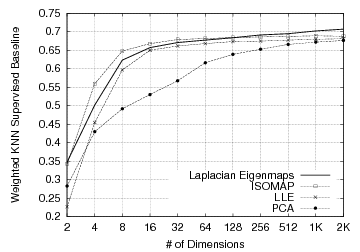
\includegraphics[width=0.5\textwidth]{baseline_graph_mono.png}
\caption{Supervised knn baselines for the four dimensionality
  reduction algorithms.}
\label{fig:dimreduce}
\end{figure}

% /scratch/esert/pos_ind/work/BASELINE_GRAPH/plot_data
% dimension PCA    LLE     ISO     LEM(Spectral)
% 2              0.2831 0.2272 0.3433 0.3480
% 4              0.4300 0.4547 0.5596 0.5019
% 8              0.4920 0.5968 0.6480 0.6234
% 16            0.5303 0.6500 0.6678 0.6572
% 32            0.5676 0.6617 0.6790 0.6708
% 64            0.6162 0.6680 0.6818 0.6774
% 128          0.6390 0.6735 0.6844 0.6838
% 256          0.6527 0.6747 0.6860 0.6914
% 512          0.6658 0.6774 0.6876 0.6948
% 1024        0.6720 0.6798 0.6891 0.7022
% 2048        0.6764 0.6811 0.6878 0.7070
% 

% this should be about same
The graph based algorithms (Isomap, LLE, and Laplacian eigenmaps) all
outperform PCA.  They stay within 5\% of their peak accuracy with as
few as 16 dimensions.  In fact Laplacian eigenmaps outperform the
baseline with the original 12,672 dimensional vectors (68.95\%) when
allowed to retain more than about 250 dimensions.  Spectral clustering
uses the same transformation as the Laplacian eigenmaps algorithm and
we compare its performance to other clustering algorithms in the next
section.

%%
  %% removed
%% % Section 3.4
%% \section{Clustering}
\label{sec:clustering}

We compared three clustering algorithms applied to the original
substitute vectors using many-to-one accuracy on the 45-tag 24K word
test corpus.  Hierarchical agglomerative clustering with complete
linkage (HAC) starts with each instance in its own cluster and
iteratively combines the two closest groups (measured by their most
distant points) at each step \cite{manning2008introduction}.
K-medoids minimizes sum of pairwise distances between each datapoint
to the exemplar at the center of its cluster
\cite{kaufman2005finding}.  Spectral clustering\footnote{We used the
  implementation in \cite{chen2011parallel} with a symmetric sparse
  affinity matrix of 550 nearest neighbors.} uses the eigenvalues of
the graph Laplacian $L=D^{-1/2} W D^{-1/2}$ to reduce the number of
dimensions (similar to Laplacian eigenmaps) and uses simple k-means
clustering on the resulting representation \cite{ng2002spectral}.  All
three algorithms accept the distance matrix based on the KL2 distance
(see Section~\ref{sec:dist}) as input.

\begin{figure}[h]
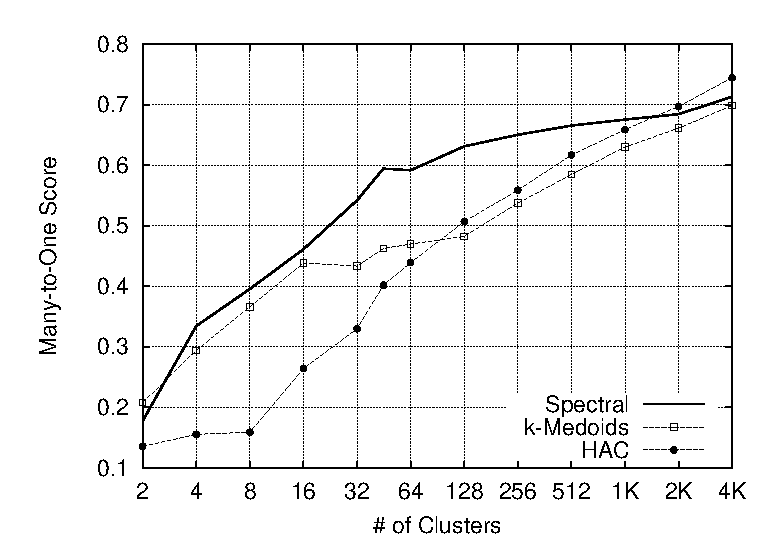
\includegraphics[width=.5\textwidth]{clustering_graph_mono.eps}
\caption{Many-to-one score for three clustering algorithms on the
  45-tag 24K word corpus.}
\label{fig:clustering}
\end{figure}

% #cluster kmedoid spectral hac
% 2          0.20795 0.17781 0.135762
% 4          0.29413 0.33439 0.155579
% 8          0.36615 0.39550 0.159076
% 16        0.43830 0.46116 0.263988
% 32        0.43318 0.54192 0.329850
% 45        0.46245 0.59413 0.401832
% 64        0.46965 0.59151 0.438843
% 128      0.48235 0.63106 0.506703
% 256      0.53709 0.65000 0.558659
% 512      0.58464 0.66520 0.616653
% 1024     0.62985 0.67523 0.658576
% 2048     0.66107 0.68414 0.696878
% 4096     0.69842 0.71286 0.744338


Figure~\ref{fig:clustering} plots the many-to-one score versus number
of clusters for the three algorithms on the 45-tag 24K word test
corpus.  The many-to-one score naturally increases as we approach the
one cluster per word limit, however we find the evolution of the
curves informative.  At the high end (more than 2000 clusters) HAC
performs best with its conservative clusters, but its performance
degrades fast as we reduce the number of clusters because it cannot
reverse the accumulating mistakes.  At the low end (less than 16
clusters) k-medoids and spectral have similar performance.  However
for the region of interest (between 16 to 2000 clusters) spectral
clustering is clearly superior with \spectralResult\% many-to-one
accuracy at 45 clusters.

  %% removed
%% Section 4, 4.1
%% \section{Co-occurrence Data Embedding}
\label{sec:code}

The general strategy we follow for unsupervised syntactic category
acquisition is to combine features of the context with the identity
and features of the target word.  Our preliminary experiments
indicated that using the context information alone (e.g. clustering
substitute vectors) without the target word identity and features had
limited success.\footnote{A 10-nearest-neighbor supervised baseline
  using cosine distance between substitute vectors gives .7213
  accuracy.  Clustering substitute vectors using various distance
  metrics and dimensionality reduction methods give results inferior
  to this upper bound.} It is the co-occurrence of a target word with a
particular type of context that best predicts the syntactic category.
In this section we review the unsupervised methods we used to model
co-occurrence statistics: the Co-occurrence Data Embedding (CODE)
method \cite{globerson2007euclidean} and its spherical extension
(S-CODE) introduced by \cite{maron2010sphere}.

Let $X$ and $Y$ be two categorical variables with finite cardinalities
$|X|$ and $|Y|$.  We observe a set of pairs $\{x_i, y_i\}_{i=1}^n$
drawn IID from the joint distribution of $X$ and $Y$.  The basic idea
behind CODE and related methods is to represent (embed) each value of
$X$ and each value of $Y$ as points in a common low dimensional
Euclidean space $\mathbf{R}^d$ such that values that frequently
co-occur lie close to each other.  There are several ways to formalize
the relationship between the distances and co-occurrence statistics, in
this paper we use the following:
\begin{equation} \label{eq:probability}
p(x,y) = \frac{1}{Z} \bar{p}(x) \bar{p}(y) e^{-d^2_{x,y}}
\end{equation}
\noindent where $d^2_{x,y}$ is the squared distance between the
embeddings of $x$ and $y$, $\bar{p}(x)$ and $\bar{p}(y)$ are empirical
probabilities, and $Z=\sum_{x,y} \bar{p}(x) \bar{p}(y) e^{-d^2_{x,y}}$ is
a normalization term.  If we use the notation $\phi_x$ for the
point corresponding to $x$ and $\psi_y$ for the point corresponding
to $y$ then $d^2_{x,y} = \|\phi_x-\psi_y\|^2$.  The log-likelihood
of a given embedding $\ell(\phi, \psi)$ can be expressed as:
\begin{eqnarray} 
&&\ell(\phi, \psi) = \sum_{x,y} \bar{p}(x,y) \log p(x,y) \label{eq:likelihood} \\
&&= \sum_{x,y} \bar{p}(x,y) (-\log Z + \log \bar{p}(x)\bar{p}(y) - d^2_{x,y}) \nonumber \\
&&= -\log Z + \mathit{const} - \sum_{x,y} \bar{p}(x,y) d^2_{x,y} \nonumber
\end{eqnarray}
The likelihood is not convex in $\phi$ and $\psi$.  We use gradient
ascent to find an approximate solution for a set of $\phi_x$, $\psi_y$
that maximize the likelihood.  The gradient of the $d^2_{x,y}$ term
pulls neighbors closer in proportion to the empirical joint
probability:
\begin{equation}
\frac{\partial}{\partial\phi_x} \sum_{x,y} -\bar{p}(x,y) d^2_{x,y} =
\sum_y 2 \bar{p}(x,y) (\psi_y - \phi_x) \label{eq:attract}
\end{equation}
The gradient of the $Z$ term pushes neighbors apart in proportion to the
estimated joint probability:
\begin{equation}
\frac{\partial}{\partial\phi_x} (-\log Z) = \sum_y 2 p(x,y) (\phi_x -
\psi_y) \label{eq:repulse}
\end{equation}
Thus the net effect is to pull pairs together if their estimated
probability is less than the empirical probability and to push them
apart otherwise.  The gradients with respect to $\psi_y$ are
similar.

S-CODE \cite{maron2010sphere} additionally restricts all $\phi_x$ and
$\psi_y$ to lie on the unit sphere.  With this restriction, $Z$ stays
around a fixed value during gradient ascent.  This allows S-CODE to
substitute an approximate constant $\tilde{Z}$ in gradient
calculations for the real $Z$ for computational efficiency.  In our
experiments, we used S-CODE with its sampling based stochastic
gradient ascent algorithm and smoothly decreasing learning
rate.


% Section 4.2 - 4.5
%%\subsection{S-Code and Substitute Vector Application}
\subsection{Experimental Settings}\label{sec:expset}

To make a meaningful comparison on the PTB we ran all the experiments
using the following default settings (unless otherwise stated): (i)
each word was kept with its original capitalization, (ii) the learning
rate parameters were set to $\varphi_0=50$, $\eta_0=0.2$ for faster
convergence in log likelihood, (iii) the number of S-CODE iterations
were set to 50 million, (iv) the S-CODE dimensions and $Z$ were set to
25 and 0.166, respectively, (v) a modified k-means algorithm with
smart initialization was used \cite{arthur2007k}, and (vi) the number
of k-means restarts were set to 128 to improve clustering and reduce
variance.

Section~\ref{sec:dist} shows that low probability substitutes are
relatively unimportant thus for computational efficiency only the top
100 substitutes and their unnormalized probabilities were computed for
each positions in the PTB(1,173,766 tokens, 49,206 types) using the
{\sc fastsubs} algorithm \cite{yuret2021fastsub}\footnote{The
  substitutes with unnormalized log probabilities can be downloaded
  from \mbox{\url{http://goo.gl/jzKH0}}.}.  The probability vectors
for each position were normalized to add up to 1.0 giving us the final
substitute vectors used in the rest of this study.  We set the
vocabulary threshold to 20 which increases the vocabulary size to
78,498.

% \footnote{Reducing the vocabulary threshold to 20 from 500

%  increases the vocabulary size to 78,498 from 12,672. }

Each experiment was repeated 10 times with different random seeds and
the results are reported with standard errors in parentheses or error
bars in graphs.  Table~\ref{tab:results} summarizes all the results
reported in this section and the ones we cite from the literature.

\subsection{Random Partitions}\label{sec:rpart}
\begin{table*}[t] \footnotesize
\caption{Summary of results in terms of the \mto and \vm scores.
  Standard errors are given in parentheses when available.  Starred
  entries have been reported in the review paper
  \protect\cite{Christodoulopoulos:2010:TDU:1870658.1870714}.  Distributional
  models use only the identity of the target word and its context.
  The models on the right incorporate orthographic and
  morphological features.}
\begin{tabular}{|@{ }l@{ }|@{ }l@{ }|@{ }l@{ }|}
\hline
Distributional Models & \mto & \vm \\
\hline
Lamar et al. \shortcite{Lamar:2010:LCU:1870658.1870736} & .708 & -\\ %algorithm name LDC
Brown et al. \shortcite{Brown:1992:CNG:176313.176316}* & .678 & .630\\
%kcls(Och,1999) & .737 & .656\\
%\cite{goldwater-griffiths:2007:ACLMain} & .632 & .562\\
Goldwater et al. \shortcite{goldwater-griffiths:2007:ACLMain} & .632 & .562\\
Ganchev et al. \shortcite{Ganchev:2010:PRS:1859890.1859918}* & .625 & .548\\
Maron et al. \shortcite{maron2010sphere} & .688 (.0016)&-\\
Bigrams (Sec.~\ref{sec:bigram}) & \bgmto & \bgvm \\
Partitions (Sec.~\ref{sec:rpart}) & \rpmto & \rpvm \\
Substitutes (Sec.~\ref{sec:wordsub}) & \wsmto & \wsvm \\
\hline
\end{tabular}
\begin{tabular}{|@{ }l@{ }|@{ }l@{ }|@{ }l@{ }|}
\hline
Models with Additional Features & \mto & \vm \\
\hline
Clark \shortcite{Clark:2003:CDM:1067807.1067817}* & .712 & .655 \\
Christodoulopoulos et al. \shortcite{christodoulopoulos-goldwater-steedman:2011:EMNLP} & .728 & .661\\
Berg-Kirkpatrick et al. \shortcite{bergkirkpatrick-klein:2010:ACL} & .755 & -\\ % Interesting in  christo paper:73.9/67.7
Christodoulopoulos et al. \shortcite{Christodoulopoulos:2010:TDU:1870658.1870714} & .761 & .688\\
Blunsom and Cohn \shortcite{blunsom-cohn:2011:ACL-HLT2011} & .775 & .697\\
Substitutes and Features (Sec.~\ref{sec:feat}) & \ftmto & \ftvm \\
& & \\
& & \\
\hline
\end{tabular}
\label{tab:results}
\end{table*}

To obtain a discrete representation of the context, the
random--partitions algorithm first designates a random subset of
substitute vectors as centroids to partition the space, and then
associates each context with the partition defined by the closest
centroid in cosine distance.  Each partition thus defined gets a
unique id, and word ($X$) -- partition-id ($Y$) pairs are given to
S-CODE as input.  The algorithm uses stochastic gradient ascent to
find the $\phi_x, \psi_y$ embeddings for word and partition-id in
these pairs on a single 25-dimensional sphere.  The algorithm cycles
through the data until we get approximately 50 million updates.  The
resulting $\phi_x$ vectors are clustered using an instance weighted
k-means algorithm and the resulting groups are compared to the correct
part-of-speech tags.  Using default settings with 64K random
partitions the many-to-one accuracy is \rpmto\ and the V-measure is
\rpvm.

To analyze the sensitivity of this result to our specific parameter
settings we ran a number of experiments where each parameter was
varied over a range of values.

\begin{figure}[ht] \centering
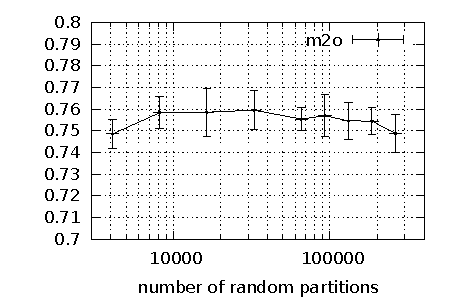
\includegraphics[width=0.5\linewidth]{plot-p.pdf}
\caption{\mto is not sensitive to the number of partitions used to
  discretize the substitute vector space within our experimental
  range.}
\label{plot-p}
\end{figure}

Figure~\ref{plot-p} gives results where the number of initial random
partitions is varied over a large range and shows the results to be
fairly stable across two orders of magnitude.

\begin{figure}[ht] \centering
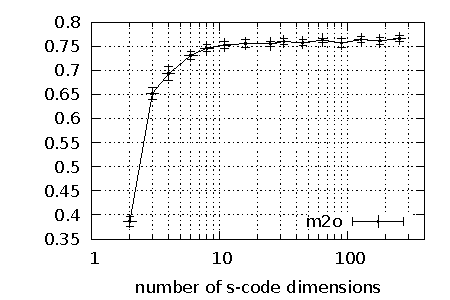
\includegraphics[width=0.5\linewidth]{plot-d.pdf}
\caption{\mto falls sharply for less than 10 S-CODE dimensions, but
  more than 25 do not help.}
\label{plot-d}
\end{figure}

Figure~\ref{plot-d} shows that at least 10 embedding dimensions are
necessary to get within 1\% of the best result, but there is no
significant gain from using more than 25 dimensions.

\begin{figure}[ht] \centering
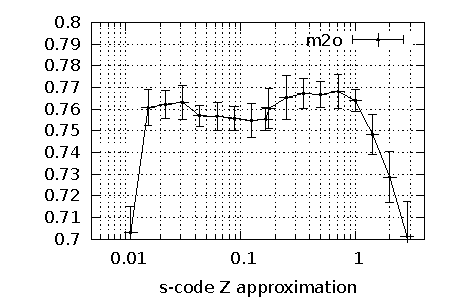
\includegraphics[width=0.5\linewidth]{plot-z.pdf}
\caption{\mto is fairly stable as long as the $\tilde{Z}$ constant is
  within an order of magnitude of the real $Z$ value.}
\label{plot-z}
\end{figure}

Figure~\ref{plot-z} shows that the constant $\tilde{Z}$ approximation
can be varied within two orders of magnitude without a significant
performance drop in the many-to-one score.  For uniformly distributed
points on a 25 dimensional sphere, the expected $Z\approx 0.146$.  In
the experiments where we tested we found the real $Z$ always to be in
the 0.140-0.170 range.  When the constant $\tilde{Z}$ estimate is too
small the attraction in Eq.~\ref{eq:attract} dominates the repulsion
in Eq.~\ref{eq:repulse} and all points tend to converge to the same
location.  When $\tilde{Z}$ is too high, it prevents meaningful
clusters from coalescing.
%%% I have seen the first, but the second is pure guess, need to
%%% look.  The distances seem to be decreasing on that end as well!

We find the random partition algorithm to be fairly robust to
different parameter settings and the resulting many-to-one score
significantly better than the state-of-the-art distributional models.

\subsection{Random Substitutes}\label{sec:wordsub}

Another way to use substitute vectors in a discrete setting is simply
to sample individual substitute words from them according to the
corresponding probabilities.  The random-substitutes algorithm cycles
through the test data and pairs each word with a random substitute
picked from the pre-computed substitute vectors (see
Section~\ref{sec:subthr}).  We ran the random-substitutes algorithm to
generate 76 million word ($X$) -- random-substitute ($Y$) pairs (64
substitutes for each token) as input to S-CODE.  Clustering the
resulting $\phi_x$ vectors yields a many-to-one score of \wsmto\ and a
V-measure of \wsvm.

This result is close to the previous result by the random-partition
algorithm, \rpmto, demonstrating that two very different discrete
representations of context based on paradigmatic features give
consistent results.  Figure~\ref{plot-s} illustrates that the
random-substitute result is fairly robust as long as the training
algorithm can observe more than a few random substitutes per word.

\begin{figure}[ht] \centering
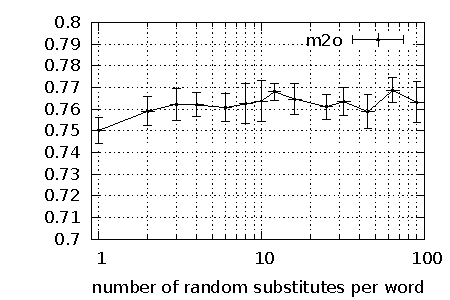
\includegraphics[width=0.5\linewidth]{plot-s.pdf}
\caption{\mto is not sensitive to the number of random substitutes
  sampled per word token.}
\label{plot-s}
\end{figure}

\subsection{Paradigmatic vs Syntagmatic Representations of Word Context}\label{sec:bigram}

To get a direct comparison of the paradigmatic and syntagmatic context
representations we feed the adjacent word pairs (bigrams) in the
corpus into the S-CODE algorithm as $X, Y$ samples
\cite{maron2010sphere} instead of pairing each word with a
paradigmatic representation of its context.  At the end each word $w$
in the vocabulary ends up with two points on the sphere, a $\phi_w$
point representing the behavior of $w$ as the left word of a bigram
and a $\psi_w$ point representing it as the right word.  The two
vectors for $w$ are concatenated to create a 50-dimensional
representation at the end.  These 50-dimensional vectors are clustered
using the k-means algorithm.  Maron et al. \shortcite{maron2010sphere}
report many-to-one scores of .6880 (.0016) for 45 clusters and .7150
(.0060) for 50 clusters (on the PTB).  If only $\phi_w$ vectors are
clustered without concatenation we found the performance drops
significantly to about .62.  Using our default settings the bigram
model achieves \bgmto \mto and \bgvm \vm accuracies.  Both results are
significantly lower than the random partition and substitute \mto and
\vm accuracies.
  %% should be copied into word-types.tex
% Section 4.6, 4.7
\section{Abstract Algorithm}

In this section we describe the components of our algorithm and their
relationship with each other.  The algorithm predicts the syntactic
category of a word in a given context based on its random substitutes.
In other words first we construct the co-occurrence representation of
words and their substitutes with the help of a language model and then
map each value in the co-occurrence data to a corresponding embedding
on a $n$-dimensional sphere using the S-CODE algorithm.  Finally, we
apply k-means clustering to categorize the word embeddings by which we
induced the word categories.  In the next subsection we detail the
representation of word contexts as co-occurrence data, in
Subsection~\ref{sec:embedding} we explain the embedding calculation
and finally in Subsection~\ref{sec:clustering} we describe the
different ways of embedding clustering.

\subsection{Context Representation}
\label{sec:cooc}
% How we represent the context?
% How we relate the word and the context?

Word contexts are represented by random substitutes that are sampled
from the corresponding substitute word distributions.  Random
substitutes are sampled with replacement from the substitute
distributions that are calculated based on an n-gram language model.
The sample space of the substitute word distributions is the
vocabulary of the language model.\footnote{Sampled substitutes might
  include the unknown word tag ``\_unk\_'' since it is in the language
  model vocabulary.  For example substitutes of proper nouns usually
  include ``\_unk\_'' as a substitute.}  It is possible (and
beneficial, see Section~\ref{sec:exp}) to sample more than one
substitutes and generate more pairs from the same substitute
distribution as in Table~\ref{tab:samples}.  The calculation of
substitute distributions and random substitute sampling are detailed
in Appendix~A.  To capture the relation between each word and its
context we construct a co-occurrence representation by pairing the
words with their random substitutes.  Table~\ref{tab:samples} shows
random substitutes of each word and their co-occurrence representation
on an example sentence.  A target word might appear as a word or a
random substitute therefore to clarify this ambiguity we concatenate
``W'' and ``C'' to words and contexts (i.e., random substitutes),
respectively, in the co-occurrence data.

The next section explains the S-CODE algorithm which takes the
co-occurrence data as its input and calculates the embeddings of the
words and their substitutes on an $n$-dimensional sphere.  In the rest
of the paper we use the term ``substitutes'' and ``random
substitutes'' interchangeably.

\begin{table}[ht]
\caption{The left table shows three possible substitutes, seperated
  with ``/'', sampled for each position in the example sentence
  \textit{``Pierre Vinken, 61 years old, will join the board as a
    nonexecutive director Nov.~29 .''} based on a 4-gram language
  model.  The right table represents the input sentence as
  co-occurrences of words and their substitutes.  Thus words on the
  left column presents the target word while words on the right column
  represents the context of the correponding target word.}
\begin{tabular}{|ll|} \hline
\textbf{Word} & \textbf{Random Substitutes}\\
\hline
Pierre & \textit{Mr.}  / \textit{Pierre} /  \textit{Mr.}\\
Vinken & \textit{\_unk\_} / \textit{Beregovoy} / \textit{Cardin}\\
, & \textit{,} / \textit{,} / \textit{,}\\
61 & \textit{48} / \textit{52} / \textit{41}\\
years & \textit{years} /  \textit{years} /  \textit{years}\\
old & \textit{old} /  \textit{old} /  \textit{old}\\
, & \textit{,} /  \textit{,} /  \textit{,}\\
will & \textit{will} /  \textit{will} /  \textit{will}\\
join & \textit{head} /  \textit{join} /  \textit{leave}\\
the  & \textit{its} /  \textit{its} /  \textit{the}\\
board & \textit{board} /  \textit{company} / \textit{firm}\\
as & \textit{as} / \textit{as} / \textit{as}\\
a & \textit{a} / \textit{a} / \textit{a}\\
nonexecutive & \textit{nonexecutive} / \textit{non-executive} / \textit{nonexecutive}\\
director & \textit{chairman} / \textit{chairman} / \textit{director}\\
Nov. & \textit{April} / \textit{May} / \textit{of}\\
29 & \textit{16} /  \textit{29} / \textit{9}\\
. & \textit{.}  / \textit{.} / \textit{.}\\
\hline
\end{tabular}
\quad
\begin{tabular}{|ll|}
\hline
\textbf{Word} & \textbf{Context}\\
\hline
W:Pierre & \textit{C:Mr.}\\
W:Pierre & \textit{C:Pierre}\\
W:Pierre & \textit{C:Mr.}\\
W:Vinken & \textit{C:\_unk\_}\\
W:Vinken & \textit{C:Beregovoy}\\
W:Vinken & \textit{C:Cardin}\\
$\hdots$&\\
W:join & \textit{C:head}\\
W:join & \textit{C:join}\\
W:join & \textit{C:leave}\\
W:the & \textit{C:its}\\
W:the & \textit{C:its}\\
W:the & \textit{C:the}\\
$\hdots$&\\
W:director & \textit{C:chairman}\\
W:director & \textit{C:chairman}\\
W:director & \textit{C:director}\\
$\hdots$&\\
\hline
\end{tabular}
\label{tab:samples}
\end{table}

\subsection{Co-occurence Embedding}
\label{sec:embedding}
The S-CODE algorithm maps each word and substitute value in the
co-occurrence data to an embedding on an $n$-dimensional sphere as
detailed in Appendix~B.  The basic idea of the mapping is that words
and substitutes that are frequently observed as pairs in the
co-occurrence data will have close embeddings while unobserved pairs
will have embeddings that are apart from each other.
\begin{figure}[ht]
\centering
  \begin{minipage}[c]{0.38\textwidth}
    \begin{tabular}{|l|l|}
    \hline
    \textbf{Word} & \textbf{Context} \\
    \hline
    $\hdots$&$\hdots$\\
    W:director & C:chairman \\
    W:chief & C:chairman \\
    $\hdots$&$\hdots$\\
    W:Pierre & C:Mr. \\
    W:Frank & C:Mr. \\
    $\hdots$&$\hdots$\\
    \hline
  \end{tabular}
  \end{minipage}
  \begin{minipage}[c]{0.48\textwidth}
    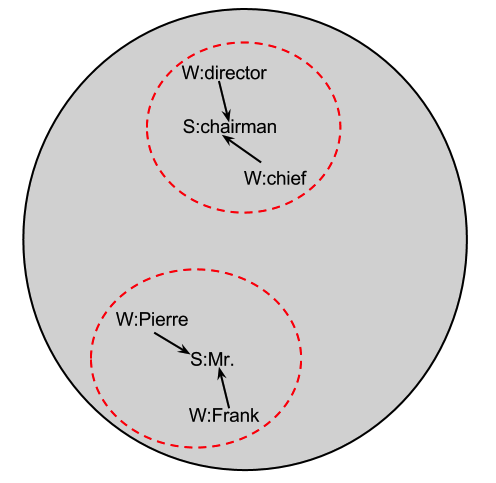
\includegraphics[height=\textwidth]{scode-ex.png}
  \end{minipage}
  \caption{The figure on the right is the final embeddings of the
    input co-occurrence data given on the left table after S-CODE
    converges.  Dashed circles represent the possible groupings of the
    embeddings on the sphere.}
  \label{fig:scodeexample}
\end{figure}

%% \begin{figure}
%% \begin{floatrow}
%% \capbtabbox{%
%% }
%% {%
%%   \caption{A co-occurrence data that
%%  is input to the S-CODE algorithm.}%
%% }
%% \hspace{1cm}
%% \ffigbox{%
%%   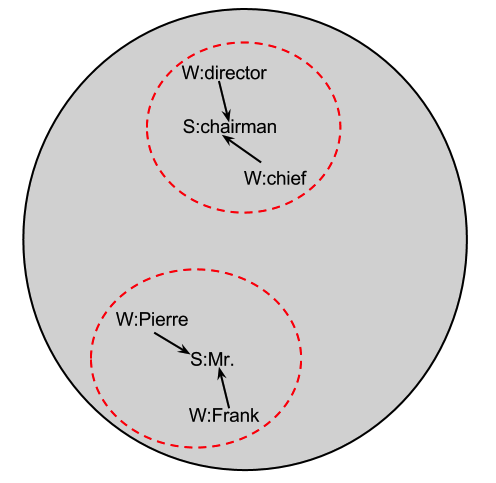
\includegraphics[height=.45\textwidth]{scode-ex.png}\\  
%% }
%% {%
%%   \caption{}  
%%   \label{fig:scodeexample}
%% }
%% \end{floatrow}
%% \end{figure}

The co-occurrence data in Figure~\ref{fig:scodeexample} consists of
pairs such as (\textit{W:director}, \textit{C:chairman}) and
(\textit{W:chief}, \textit{C:chairman}) therefore S-CODE forces the
embeddings of \textit{W:director} and \textit{W:chief} to be close to
the embedding of \textit{C:chairman}.  Similar to the former case the
embeddings of \textit{W:Pierre} and \textit{W:Frank} will be close to
the embedding \textit{C:Mr.} becouse of the frequently observed pairs.
As a results the final embeddings of \textit{W:director} and
\textit{W:chief} will be close to each other due to the common
substitute \textit{C:chairman} and will be apart from
\textit{W:Pierre} and \textit{W:Frank} due to the lack of common
substitute as shown on Figure~\ref{fig:scodeexample} (similarly the
embeddings of \textit{W:Pierre} and \textit{W:Frank} will be close to
each other due to \textit{C:Mr.}).

% How we relate final embeddings and the input pairs?
S-CODE constructs embeddings on $n$-dimensional sphere for each unique
value of words and substitutes.  Thus each pair in the co-occurrence
data can be represented in three different ways by using the output of
S-CODE: (1) word embedding (${\bf W}$) which represents the word type
information, (2) substitute embedding (${\bf C}$) which represents the
context information, and (3) word and substitute embeddings
concatenated (${\bf W}\oplus{\bf C}$).  In the next section we apply
k-means clustering to these three representation and analyze the
characteristic of final clusters.

\subsection{Embedding Clustering}
\label{sec:clustering}
%% In Section~\ref{sec:cooc} we decribe the tranformation of an input
%% sentence to a co-occurrence data and we represent each target word
%% with the word--substitute pair(s).  In the previous section we
%% construct embeddings for each value observed in the co-occurrence data
%% using the S-CODE algorithm. 

Each target word in the original input sentence is represented with
word--substitute pairs and each unique word and substitute value are
represented with embeddings on an $n$ dimensional sphere.  Therefore
clustering the embeddings means clustering the target words in the
original input.  We run instance weighted k-means algorithm to cluster
the final embeddings constructed by S-CODE.  The target words can be
represented in three ways as described in the previous section.
Clustering each representation with k-means will end up with a
clusters with different characteristics.

\paragraph{Word embeddings (${\bf W}$)} All of the target word
instances are represented with the same embedding.  For instance,
although we sample three substitutes per target word in
Table~\ref{tab:samples}, each unique target word has only one
embedding in ${\bf W}$.  Thus clustering target words based on this
representation employ the one-tag-per-word assumption from the
beginning.  The one-tag-per-word assumption is suitable for the part
of speech induction problem given that 93.69\% of the word occurrences
in the human labeled PTB data are tagged with their most frequent part
of speech \cite{Toutanova:2003:FPT:1073445.1073478}.  However the
clustering performance on the ambiguous words (words that have more
than one tag) degrades due to the one-tag-per-word assumption.  For
example, the word ``offer'' is tagged as NN(399), VB(105) and VBP(34)
in its 538 WSJ instances\footnote{NN, VB and VBP are three
  part-of-speech tags from the Penn Treebank corpus and they
  correspond to singular noun, verb in base form and
  non-$3^{rd}$person singular verb in present tense, respectively.}.
In this scheme all instances of ``offer'' tagged with one tag and the
\mto\ upper bound accurcy of ``offer'' is .7616 since the most
frequent tag is NN(399). Our model in Section~\ref{sec:clustering-w}
clusters word embeddings and achieves the \mto\ upper bound of
``offer'' however this is not the case for all ambiguous words.

%offer tag distribution in WSJ VBP 34, VB 105, NN 399
\paragraph{Context embeddings (${\bf C}$)} 
Each target word instance is represented with embeddings of its
substitutes instead of its word embedding therefore clustering them
does not employ or force the one-tag-per-word assumption.  For
example, the word ``Pierre'' in Table~\ref{tab:samples} will be
represented with the embeddings of {\it S:Mr.}, {\it S:Pierre} and
{\it S:Mr.}  however another occurrence of the word ``Pierre'' in a
different context might be represented with different substitutes.  It
is possible to represent context with several substitutes, in such a
case k-means might group substitute embeddings into different clusters
which leads to an ambiguity on the final cluster of the target word.
To solve this issue the target word is assigned to the cluster in
which the majority of its substitute embeddings are
present\footnote{Ties are broken randomly.}.  The model in
Section~\ref{sec:clustering-c} clusters ${\bf C}$ and achieves .8215
\mto\ on the word ``offer'' which is higher than the one-tag-per-word
\mto\ upper bound.

\paragraph{Concatenation word and context embeddings (${\bf W\oplus C}$)} 
This representation concatenates the word and its substitute
embeddings such that each target word is represented with $r$ vectors
where $r$ is the number of random substitutes per target word.
Therefore it explicitly forces the one-tag-per-word assumption while
handling the ambiguity.  For instance, the target word ``Pierre'' in
Table~\ref{tab:samples} will be represented with three vectors that
will be the concatenation of the embedding of {\it W:Pierre} with the
embeddings of {\it C:Mr.}, {\it C:Pierre} and {\it C:Mr.}, seperately.
Similar to the former case we run k-means clustering on these
concatenated vectors and use majority voting to assign the target word
cluster.  The model in Section~\ref{sec:clustering-concatenation}
handles the ambiguity while using the fact that words are observed
with their most frequent POS tag and outperforms the previous models
by scoring .8866 \mto\ accuracy on the word ``offer''.

The first representation applies the one-tag-per-word assumption from
the beginning and clusters word types instead of tokens.  On the other
hand the second one relaxes the one-tag-per-word assumption and
clusters word tokens.  The final one also clusters tokens however it
represents each token with the concatenation of the word and context
embeddings therefore it forces the one-tag-per-word assumption while
handling the ambiguity.  Section~\ref{sec:exp} compares the
performance of these three representations on the word category
induction problem.

%\subsection{S-Code and Substitute Vector Application}
\subsection{Experimental Settings}\label{sec:expset}

To make a meaningful comparison on the PTB we ran all the experiments
using the following default settings (unless otherwise stated): (i)
each word was kept with its original capitalization, (ii) the learning
rate parameters were set to $\varphi_0=50$, $\eta_0=0.2$ for faster
convergence in log likelihood, (iii) the number of S-CODE iterations
were set to 50 million, (iv) the S-CODE dimensions and $Z$ were set to
25 and 0.166, respectively, (v) a modified k-means algorithm with
smart initialization was used \cite{arthur2007k}, and (vi) the number
of k-means restarts were set to 128 to improve clustering and reduce
variance.

Section~\ref{sec:dist} shows that low probability substitutes are
relatively unimportant thus for computational efficiency only the top
100 substitutes and their unnormalized probabilities were computed for
each positions in the PTB(1,173,766 tokens, 49,206 types) using the
{\sc fastsubs} algorithm \cite{yuret2021fastsub}\footnote{The
  substitutes with unnormalized log probabilities can be downloaded
  from \mbox{\url{http://goo.gl/jzKH0}}.}.  The probability vectors
for each position were normalized to add up to 1.0 giving us the final
substitute vectors used in the rest of this study.  We set the
vocabulary threshold to 20 which increases the vocabulary size to
78,498.

% \footnote{Reducing the vocabulary threshold to 20 from 500

%  increases the vocabulary size to 78,498 from 12,672. }

Each experiment was repeated 10 times with different random seeds and
the results are reported with standard errors in parentheses or error
bars in graphs.  Table~\ref{tab:results} summarizes all the results
reported in this section and the ones we cite from the literature.

\subsection{Random Partitions}\label{sec:rpart}
\begin{table*}[t] \footnotesize
\caption{Summary of results in terms of the \mto and \vm scores.
  Standard errors are given in parentheses when available.  Starred
  entries have been reported in the review paper
  \protect\cite{Christodoulopoulos:2010:TDU:1870658.1870714}.  Distributional
  models use only the identity of the target word and its context.
  The models on the right incorporate orthographic and
  morphological features.}
\begin{tabular}{|@{ }l@{ }|@{ }l@{ }|@{ }l@{ }|}
\hline
Distributional Models & \mto & \vm \\
\hline
Lamar et al. \shortcite{Lamar:2010:LCU:1870658.1870736} & .708 & -\\ %algorithm name LDC
Brown et al. \shortcite{Brown:1992:CNG:176313.176316}* & .678 & .630\\
%kcls(Och,1999) & .737 & .656\\
%\cite{goldwater-griffiths:2007:ACLMain} & .632 & .562\\
Goldwater et al. \shortcite{goldwater-griffiths:2007:ACLMain} & .632 & .562\\
Ganchev et al. \shortcite{Ganchev:2010:PRS:1859890.1859918}* & .625 & .548\\
Maron et al. \shortcite{maron2010sphere} & .688 (.0016)&-\\
Bigrams (Sec.~\ref{sec:bigram}) & \bgmto & \bgvm \\
Partitions (Sec.~\ref{sec:rpart}) & \rpmto & \rpvm \\
Substitutes (Sec.~\ref{sec:wordsub}) & \wsmto & \wsvm \\
\hline
\end{tabular}
\begin{tabular}{|@{ }l@{ }|@{ }l@{ }|@{ }l@{ }|}
\hline
Models with Additional Features & \mto & \vm \\
\hline
Clark \shortcite{Clark:2003:CDM:1067807.1067817}* & .712 & .655 \\
Christodoulopoulos et al. \shortcite{christodoulopoulos-goldwater-steedman:2011:EMNLP} & .728 & .661\\
Berg-Kirkpatrick et al. \shortcite{bergkirkpatrick-klein:2010:ACL} & .755 & -\\ % Interesting in  christo paper:73.9/67.7
Christodoulopoulos et al. \shortcite{Christodoulopoulos:2010:TDU:1870658.1870714} & .761 & .688\\
Blunsom and Cohn \shortcite{blunsom-cohn:2011:ACL-HLT2011} & .775 & .697\\
Substitutes and Features (Sec.~\ref{sec:feat}) & \ftmto & \ftvm \\
& & \\
& & \\
\hline
\end{tabular}
\label{tab:results}
\end{table*}

To obtain a discrete representation of the context, the
random--partitions algorithm first designates a random subset of
substitute vectors as centroids to partition the space, and then
associates each context with the partition defined by the closest
centroid in cosine distance.  Each partition thus defined gets a
unique id, and word ($X$) -- partition-id ($Y$) pairs are given to
S-CODE as input.  The algorithm uses stochastic gradient ascent to
find the $\phi_x, \psi_y$ embeddings for word and partition-id in
these pairs on a single 25-dimensional sphere.  The algorithm cycles
through the data until we get approximately 50 million updates.  The
resulting $\phi_x$ vectors are clustered using an instance weighted
k-means algorithm and the resulting groups are compared to the correct
part-of-speech tags.  Using default settings with 64K random
partitions the many-to-one accuracy is \rpmto\ and the V-measure is
\rpvm.

To analyze the sensitivity of this result to our specific parameter
settings we ran a number of experiments where each parameter was
varied over a range of values.

\begin{figure}[ht] \centering
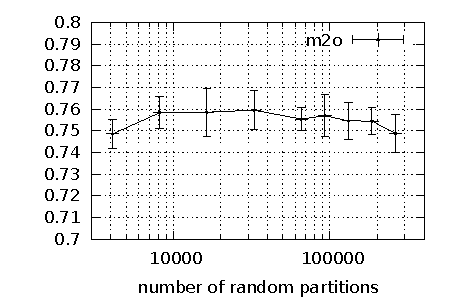
\includegraphics[width=0.5\linewidth]{plot-p.pdf}
\caption{\mto is not sensitive to the number of partitions used to
  discretize the substitute vector space within our experimental
  range.}
\label{plot-p}
\end{figure}

Figure~\ref{plot-p} gives results where the number of initial random
partitions is varied over a large range and shows the results to be
fairly stable across two orders of magnitude.

\begin{figure}[ht] \centering
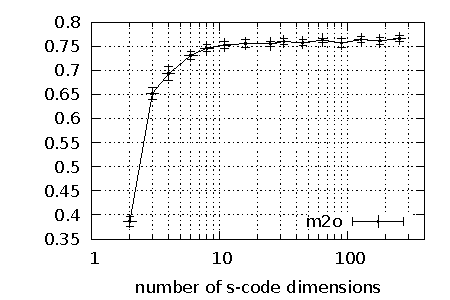
\includegraphics[width=0.5\linewidth]{plot-d.pdf}
\caption{\mto falls sharply for less than 10 S-CODE dimensions, but
  more than 25 do not help.}
\label{plot-d}
\end{figure}

Figure~\ref{plot-d} shows that at least 10 embedding dimensions are
necessary to get within 1\% of the best result, but there is no
significant gain from using more than 25 dimensions.

\begin{figure}[ht] \centering
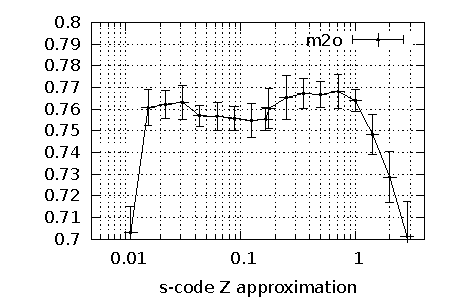
\includegraphics[width=0.5\linewidth]{plot-z.pdf}
\caption{\mto is fairly stable as long as the $\tilde{Z}$ constant is
  within an order of magnitude of the real $Z$ value.}
\label{plot-z}
\end{figure}

Figure~\ref{plot-z} shows that the constant $\tilde{Z}$ approximation
can be varied within two orders of magnitude without a significant
performance drop in the many-to-one score.  For uniformly distributed
points on a 25 dimensional sphere, the expected $Z\approx 0.146$.  In
the experiments where we tested we found the real $Z$ always to be in
the 0.140-0.170 range.  When the constant $\tilde{Z}$ estimate is too
small the attraction in Eq.~\ref{eq:attract} dominates the repulsion
in Eq.~\ref{eq:repulse} and all points tend to converge to the same
location.  When $\tilde{Z}$ is too high, it prevents meaningful
clusters from coalescing.
%%% I have seen the first, but the second is pure guess, need to
%%% look.  The distances seem to be decreasing on that end as well!

We find the random partition algorithm to be fairly robust to
different parameter settings and the resulting many-to-one score
significantly better than the state-of-the-art distributional models.

\subsection{Random Substitutes}\label{sec:wordsub}

Another way to use substitute vectors in a discrete setting is simply
to sample individual substitute words from them according to the
corresponding probabilities.  The random-substitutes algorithm cycles
through the test data and pairs each word with a random substitute
picked from the pre-computed substitute vectors (see
Section~\ref{sec:subthr}).  We ran the random-substitutes algorithm to
generate 76 million word ($X$) -- random-substitute ($Y$) pairs (64
substitutes for each token) as input to S-CODE.  Clustering the
resulting $\phi_x$ vectors yields a many-to-one score of \wsmto\ and a
V-measure of \wsvm.

This result is close to the previous result by the random-partition
algorithm, \rpmto, demonstrating that two very different discrete
representations of context based on paradigmatic features give
consistent results.  Figure~\ref{plot-s} illustrates that the
random-substitute result is fairly robust as long as the training
algorithm can observe more than a few random substitutes per word.

\begin{figure}[ht] \centering
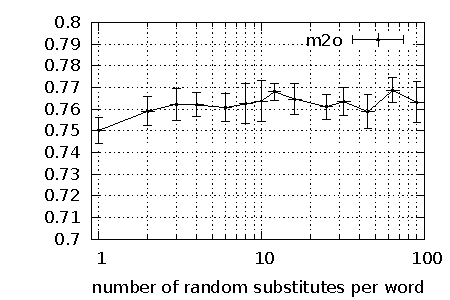
\includegraphics[width=0.5\linewidth]{plot-s.pdf}
\caption{\mto is not sensitive to the number of random substitutes
  sampled per word token.}
\label{plot-s}
\end{figure}

\subsection{Paradigmatic vs Syntagmatic Representations of Word Context}\label{sec:bigram}

To get a direct comparison of the paradigmatic and syntagmatic context
representations we feed the adjacent word pairs (bigrams) in the
corpus into the S-CODE algorithm as $X, Y$ samples
\cite{maron2010sphere} instead of pairing each word with a
paradigmatic representation of its context.  At the end each word $w$
in the vocabulary ends up with two points on the sphere, a $\phi_w$
point representing the behavior of $w$ as the left word of a bigram
and a $\psi_w$ point representing it as the right word.  The two
vectors for $w$ are concatenated to create a 50-dimensional
representation at the end.  These 50-dimensional vectors are clustered
using the k-means algorithm.  Maron et al. \shortcite{maron2010sphere}
report many-to-one scores of .6880 (.0016) for 45 clusters and .7150
(.0060) for 50 clusters (on the PTB).  If only $\phi_w$ vectors are
clustered without concatenation we found the performance drops
significantly to about .62.  Using our default settings the bigram
model achieves \bgmto \mto and \bgvm \vm accuracies.  Both results are
significantly lower than the random partition and substitute \mto and
\vm accuracies.

\subsection{Clustering Context Embeddings (${\bf C}$)}
\label{sec:clustering-c}

In the previous section we group word types rather than word tokens by
clustering the word embeddings.  In this section we remove the
one-tag-per-word assumption and group word tokens according to
embeddings of their substitutes.  We generate 64 substitutes for each
word token and input them to S-CODE as word($W$) -- substitute (${\bf C}$)
pairs.  The resulting embeddings of the context (i.e., substitutes)
are clustered using the instance weighted k-means algorithm with 128
restarts.  The process yields 64 cluster-ids (for every pair generated
from word token's context) for each word token's context.  The
cluster-ids tokens are predicted by the majority cluster-id of the
corresponding pairs.  Ties for the majority are broken randomly.  The
many-to-one accuracy is \wsymto\ and the V-measure is \wsyvm\ .

In order to demonstrate the merit in the token based POS induction, we
first define the gold-tag perplexity for the word types as following:
\begin{equation} \label{eq:tag-perp}
GP(w) = 2^{H(p_w)} = 2^{-\sum_{t} p_w(t)log_2 p_w(t)}
\end{equation}
\noindent where $p_w$ is the gold POS tag distribution of the word
type $w$ and $H(p_w)$ is the entropy of the $p_w$ distribution.
Gold-tag perplexity ($GP$) is used to determine the POS ambiguity of
the word types, relating how often a word type is associated with
different POS tags in the test corpus.  A $GP$ of 1 for a word type
$w$ indicates $w$ is associated with same POS tag throughout the test
corpus, meaning the word type $w$'s POS is unambiguous.  As the $GP$
increases ambiguity of the word types increases and poses a handicap
for induction models that limits tag variety for the word types.  To
display the limitations, we split the test corpus in two subsets: word
types with $GP$ less than 1.75 and word types with $GP$ equal or
greater than 1.75.  We performed \mto\ evaluation on our induction
output and obtained the induced-tag -- gold-tag mappings. Using the
mappings obtained over the test corpus, we evaluated the accuracy in
the subsets. 

\begin{table}[h]
  \small
  \centering
  \caption{The \mto\ accuracy of ${\bf W}$, ${\bf C}$ and ${\bf W}\oplus{\bf C}$
    based models on two subsets that consist of words with $GP$ smaller
    and larger than 1.75, respectively.  The
    percentage of each subset in the test data is reported in the title
    bar.  The average $GP$ of each
    clustering over the whole corpus is reported in the last column.  Each
    score is an average of 10 random starts of our algorithm and the
    standard error of each one is reported in parenthesis while
    statistically the best \mto\ score of each column is reported in bold.  
  }
  \label{tab:bins}
  \begin{tabular}{|c|c|c|c||c|}
    \hline
    Model & \specialcell{$GP < 1.75$\\$89\%$} & \specialcell{$GP \ge 1.75$\\$11\%$} & \specialcell{$GP \ge 1$ \\ $100\%$} & Average $GP$ \\
    \hline
    \specialcell{Clustering ${\bf W}$ embeddings\\(Type based)} & {\bf .8054 (.0065)} & .4383 (.0104) & {\bf \wsmto} & 1.0 (.0)\\
    \hline
    \specialcell{Clustering ${\bf W} \oplus {\bf C}$ embeddings\\(Sparse-token based)}& .7322 (.0079) & {\bf .4671 (.0174)} & \wsxymto & 1.3406 (.0057)\\ 
    \hline
    \specialcell{Clustering ${\bf C}$ embeddings\\(Token based)} & .6620 (.0051) & .4309 (.0093) & \wsymto & 1.5318 (.0076)\\
    \hline  
  \end{tabular}
\end{table}

The performance of our algorithm on ${\bf C}$ embeddings is summarized
in Table~\ref{tab:bins}.  Due to the one-tag-per-word nature of POS
induction, the type based model outperforms the token based one on the
unambiguous words. The token based model achieves statistically
comparable results with the type based model on the ambiguous words.
Type based model can not handle words with ambiguity while the token
based model can.  In order to take advantage of both models we apply
our algorithm on concatenation of ${\bf W}$ and ${\bf C}$ embeddings
in the next section.

\subsection{Clustering Concatenation of Word and Context Embeddings (${\bf W}\oplus{\bf C}$)}
\label{sec:clustering-concatenation}

Two models presented in earlier sections perform POS induction either
by assuming (Section~\ref{sec:clustering-w}) or discarding
(Section~\ref{sec:clustering-c}) the one-tag-per-word assumption.  In
this section we define a sparse-token based model which clusters the
concatenation of ${\bf W}$ and ${\bf C}$ embeddings.  This model not
only tends to put instances of a word type into the same cluster but
also performs token based clustering by incorporating the word type
and context information together.

Similar to the previous models, we generate ${\bf W}$ -- ${\bf C}$
pairs as the input to S-CODE.  For each observed ${\bf W}$ -- ${\bf
  C}$ pair in the S-CODE input, corresponding 25-dimensional $\phi_w$
and $\psi_c$ embeddings are concatenated to create a 50-dimensional
representation.  We used the same experimental setting of the previous
section and predict the token clusters according to the majority
cluster-id of the corresponding pairs.  The many-to-one accuracy of
this model is \wsxymto\ and the V-measure is \wsxyvm\ .

Table~\ref{tab:bins} presents the performance of the ${\bf
  W}\oplus{\bf C}$ based model over the subsets and it achieves
statistically better \mto\ than both of the ${\bf W}$ and ${\bf C}$
based models on ambiguous words.  Due to the bias towards to the
sparse clustering, sparse-token based model statistically improves the
\mto\ accuracy on unambiguous words compared to the ${\bf C}$ based
model but it still can not achieve the performance of the ${\bf W}$
based model.  The ${\bf W}\oplus{\bf C}$ based model constructs token
based clusters that tend to assign instances of a word type into the
same cluster which leads to a smaller average $GP$ than the ${\bf C}$
based model as shown in Table~\ref{tab:bins}.

%% We don't really need this part
%% \subsubsection{Paradigmatic vs Syntagmatic Representations of Word Context}
%% \label{sec:bigram-token}
%% In order to compare the token clustering performance of the
%% paradigmatic and the syntagmatic context representations we use the
%% same 4 models defined in Section~\ref{sec:bigram-type}.  Following the
%% previous section we concatenate the 25-dimensional $\phi_x$ and
%% $\psi_y$ ($\psi_{y_{1}}$ and $\psi_{y_{2}}$ in the fourth model)
%% embeddings of the corresponding observed pairs (tuples in the fourth
%% model) and represent the first three models outputs with a
%% 50-dimensional vectors (75-dimensional vectors in the fourth model).
%% The resulting vectors are clustered using k-means algorithm with 128
%% restarts.
%% \begin{table}[ht]
%% \centering
%% \small
%% \caption{Accuracies of the token based S-CODE models on the gold-tag
%%   perplexity separated subsets.}
%% \begin{tabular}{|l|l|l|l|}
%% \hline
%% Model & \specialcell{$GP < 1.75$\\$89\%$} & \specialcell{$GP \ge 1.75$\\$11\%$} & \specialcell{$GP \ge 1.0$\\$100\%$}\\
%% \hline
%% $X$ (word) - $Y$ (left bigram) & .5950 (.0051) & .4783 (.0005) & .5821 (.0041)\\
%% $X$ (word) - $Y$ (right bigram) & .6239 (.0049) & .3075 (.0153) & .5891 (.0046)\\
%% $X$ (word) - $Y$ (left and right bigram concatenation) & .7523 (.0065) & .4492 (.0240) & .7190 (.0049)\\
%% $X$ (word) - $Y_1$, $Y_2$ (left and right bigrams) & .6697 (.0065) & .4579 (.0052) & .6464 (.0051)\\
%% $X$ (word) - $Y$ (random substitutes) & .7322 (.0079) & .4671 (.0174) & .7030 (.0073)\\
%% \hline
%% \end{tabular}
%% \label{tab:tokens}
%% \end{table}

\subsection{Morphological and orthographic features}\label{sec:feat}

Clark \shortcite{Clark:2003:CDM:1067807.1067817} demonstrates that
using morphological and orthographic features significantly improves
part-of-speech induction with an HMM based model.
Section~\ref{sec:related} describes a number other approaches that
show similar improvements.  This section describes one way to
integrate additional features to the random-substitute model.

In order to accommodate multiple feature types the CODE model needs to
be extended to handle more than two variables.
\cite{globerson2007euclidean} suggest the following likelihood
function:

\begin{eqnarray}
&\ell(\phi,& \psi^{(1)}, \ldots, \psi^{(K)}) = \label{eq:multiscode}\\
&&\sum_k w_k \sum_{x,y^{(k)}} \bar{p}(x,y^{(k)}) \log p(x,y^{(k)}) \nonumber
\end{eqnarray}

\noindent where $Y^{(1)}, \ldots, Y^{(K)}$ are $K$ different variables
whose empirical joint distributions with $X$,
$\bar{p}(x,y^{(1)})\ldots\bar{p}(x,y^{(K)})$, are known.
Eq.~\ref{eq:multiscode} then represents a set of CODE models
$p(x,y^{(k)})$ where each $Y^{(k)}$ has an embedding $\psi_y^{(k)}$
but all models share the same $\phi_x$ embedding.  The weights $w_k$
reflect the relative importance of each $Y^{(k)}$ and all embeddings
are mapped to unit-sphere to fix the $Z^{(k)}$ around a fix value.

We adopt this likelihood function, set all $w_k=1$, let $X$
represent a word, $Y^{(1)}$ represent a random substitute and
$Y^{(2)}, \ldots, Y^{(K)}$ stand for various morphological and
orthographic features of the word.  With this setup, the training
procedure needs to change little: each time a word --
random-substitute pair is sampled, the relevant word -- feature pairs
are also generated and input to the gradient ascent algorithm.

One problem with this setup is, unobserved features misguide the
gradient search algorithm and lead to a suboptimal convergence point.
For example, ``\textbf{car}'' and ``\textbf{red}'' belong to the ``Noun''
and ``Adjective'' clusters, respectivly, and neither of them have a
morphological feature, thus their morphological features are
represented by a null value, ``X''.  However setting the unobserved
features of words from different clusters to ``X'' leads to a false
similarity between these words.  To solve this problem, during the
gradient search we don't perform any pull or push updates on
embeddings if the corresponding $y^{(k)}$ is null\footnote{$x\inX$
  represents a word type therefore it is always observed.}.

The orthographic features we used are similar to the ones in
\cite{bergkirkpatrick-EtAl:2010:NAACLHLT} with small modifications:

\begin{itemize}
\item Initial-Capital: this feature is generated for capitalized words
  with the exception of sentence initial words.
\item Number: this feature is generated when the token starts with a
  digit.
\item Contains-Hyphen: this feature is generated for lowercase words
  with an internal hyphen.
\item Initial-Apostrophe: this feature is generated for tokens that
  start with an apostrophe.
\end{itemize}

We generated morphological features using the unsupervised algorithm
Morfessor \cite{creutz05}.  Morfessor was trained on the WSJ section
of the Penn Treebank using default settings, and a perplexity
threshold of 1.  In our model, a word type consists of two parts: a
stem and a suffix part.  The suffix parts are used as the
morphological feature thus each word type has only one morphological
feature.  We extracted the stem part by concatinating the splits until
including the first ``STM'' labeled split and the suffix part by
concatinating rest of the splits\footnote{The program induced 5575
  suffix types that are present in a total of 19223 word types.}.

%% These suffixes were input to S-CODE as morphological features whenever
%% the associated word types were sampled.  In order to incorporate
%% morphological and orthographic features into
%% S-CODE we modified its input.  For each word -- random-substitute pair
%% generated as in the previous section, we added word -- feature pairs
%% to the input for each morphological and orthographic feature of the
%% word.  Words on average have 0.25 features associated with them.
%% This increased the number of pairs input to S-CODE from 14.1
%% million (12 substitutes per word) to 17.7 million (additional 0.25
%% features on average for each of the 14.1 million words).

Using similar training settings as the previous section, the addition
of morphological and orthographic features increased the many-to-one
score of the random-substitute model to \ftmto\ and V-measure to \ftvm.
Both these results improve the state-of-the-art in part-of-speech
induction significantly as seen in Table~\ref{tab:results}.

\begin{figure*}[ht] \centering
%\vspace*{-10mm}
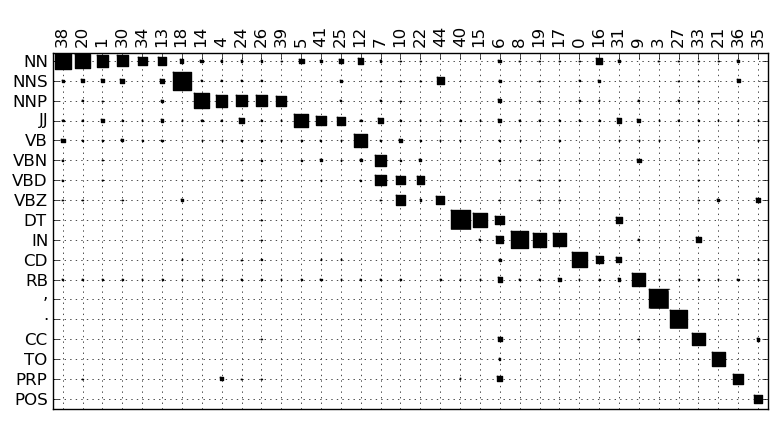
\includegraphics[width=\textwidth]{hinton.png}
%\vspace*{-30mm}
\caption{Hinton diagram comparing most frequent tags and clusters.}
\label{plot-hinton}
\end{figure*}


\subsection{Paradigmatic vs Syntagmatic Representations of Word Context}
\label{sec:pvss}

To get a direct comparison of the paradigmatic and syntagmatic context
representations we feed 4 different co-occurrences defined in
Section~\ref{sec:representation} into the S-CODE algorithm.  The first
model accepts word ($X$) - right bigram ($Y$) pairs as the input, the
second model accepts word ($X$) - left bigram($Y$) pairs as the input,
the third model accepts word ($X$) - concatenation of the left and
right bigrams ($Y$) pairs \cite{mintz2003frequent} as the input and
the final model accepts words ($X$) - left bigram($Y_1$) and right
bigram ($Y_2$) tuples \cite{20674613} as the input to the S-CODE.  At
the end we cluster the word types ($X$) with k-means algorithm and
report the results on Table \ref{tab:syntagmatic}.
\begin{table}[ht]
\centering
\caption{Summary of results in terms of the \mto\ and \vm\ scores of
  the S-CODE algorithm when the paradigmatic or syntagmatic
  representations are feed as an input.  Standard errors are given in
  parentheses when available.  Results of the statistically best
  performing system are written in bold.  We do not report the
  original results of Maron et al. \protect\shortcite{maron2010sphere}
  since our replication achieves higher accuracies.}
\begin{tabular}{|l|l|l|}
\hline
Input & \mto & \vm\\
\hline
$X$ (word) - $Y$ (right bigram) & .6625 (.0115) & .5809 (.0066)\\
$X$ (word) - $Y$ (left bigram) & .6604 (.0054) & .5983 (.0028)\\
$X$ (word) - $Y$ (left and right bigram concatenation) & .7268 (.0091) & .6416 (.0052)\\
$X$ (word) - $Y_1$, $Y_2$ (left and right bigrams) & .7173 (.0061) & .6381 (.0032)\\
Maron et al. \shortcite{maron2010sphere}(replication)  & \bgmto & \bgvm \\
$X$ (word) - $Y$ (random substitutes) & {\bf\wsmto} & {\bf\wsvm} \\
\hline
\end{tabular}
\label{tab:syntagmatic}
\end{table}
To replicate the work of Maron et al. \shortcite{maron2010sphere} we
feed word ($X$) - right bigram ($Y$) pairs as the input.  At the end
each word $w$ in the vocabulary ends up with two points on the sphere,
a $\phi_w$ point representing the behavior of $w$ as the left word of
a bigram and a $\psi_w$ point representing it as the right word.  The
two vectors for $w$ are concatenated to create a 50-dimensional
representation at the end.  These 50-dimensional vectors are clustered
using the k-means algorithm.  Maron et al. \shortcite{maron2010sphere}
report many-to-one scores of .6880 (.0016) for 45 clusters and .7150
(.0060) for 50 clusters (on the PTB).  Using our default settings the
bigram model achieves \bgmto\ \mto\ and \bgvm\ \vm\ accuracies.  Table
\ref{tab:syntagmatic} summarizes all the results and shows that the
paradigmatic representation accuracies are significantly higher than
the syntagmatic representation \mto\ and \vm\ accuracies.

\section{Multiple Languages}
\begin{landscape}
%%Multiple laguage section
\begin{table}[ht]
  \begin{tabular}{|l|l|l|p{2cm}|p{2cm}|p{2cm}|p{2cm}|p{2cm}|p{2cm}|p{2cm}|}
        \hline
        Language   & Types   & Tags & k-means      & SVD2         & clark        & BMMM         & PYP-1HMM-LM & uPos Letter Features & uPos     \\ \hline % Multext data
        English    & 49,190  & 45   & 59.5 / 61.6   & 58.2 / 64.0   & 65.6 / 71.2   & 66.1 / 72.8   & 69.7 / 77.5 & ~               & \wsvm / \wsmto           \\ \hline
        Bulgarian  & 16,352  & 12+1 & 50.3 / 59.3   & 41.7 / 51.0   & 55.6 / 66.5   & 54.5 / 64.4   & -           & 55.1 / 70.7     & 53.3 / 69.4 \\
        Czech      & 19,115  & 12+1 & 48.6 / 56.7   & 35.5 / 50.9   & 52.6 / 64.1   & 53.9 / 64.2   & -           & 47.9 / 67.0     & 47.2 / 66.9 \\
        English    & 9,773   & 12+1 & 56.5 / 65.4   & 52.3 / 65.5   & 60.5 / 70.6   & 63.3 / 73.3   & -           & 67.1 / 82.9     & 66.6 / 83.2 \\
        Estonian   & 17,845  & 12+1 & 45.3 / 55.6   & 38.7 / 55.3   & 44.4 / 58.4   & 53.3 / 64.4   & -           & 44.9 / 65.4     & 43.4 / 65.1 \\
        Hungarian  & 20,321  & 11+1 & 46.7 / 53.9   & 39.8 / 49.5   & 48.9 / 61.4   & 54.8 / 68.2   & -           & 51.9 / 70.2     & 49.6 / 68.6 \\
        Romanian   & 15,189  & 12+1 & 45.2 / 55.1   & 42.1 / 52.6   & 40.9 / 49.9   & 52.3 / 61.1   & -           & 51.9 / 65.9     & 49.5 / 64.3 \\
        Slovene    & 17,871  & 12+1 & 46.9 / 56.2   & 39.5 / 54.2   & 54.9 / 69.4   & 56.7 / 67.9   & -           & 49.1 / 69.2     & 47.4 / 68.0 \\
        Serbian    & 18,095  & 12+1 & 41.4 / 47.0   & 39.1 / 54.6   & 51.0 / 64.1   & 49.0 / 62.0   & -           & 43.7 / 61.3     & 44.4 / 62.4 \\
        Arabic     & 12,915  & 20   & 43.3 / 60.7   & 27.6 / 49.0   & 40.6 / 59.8   & 42.4 / 61.5   & - / 67.5    & -               & -           \\ \hline % Conll06 data
        Bulgarian  & 32,439  & 54   & 53.6 / 65.6   & 49.0 / 65.3   & 59.6 / 70.4   & 58.8 / 68.9   & - / 73.2    & 57.9 / 73.4     & 57.5 / 73.2 \\
        Chinese    & 40,562  & 15   & 32.6 / 61.1   & 24.5 / 54.6   & 31.8 / 56.7   & 42.6 / 69.4   & -           & -               & -           \\
        Czech      & 130,208 & 12   & -             & -            & 47.1 / 65.5   & 48.4 / 65.7    & - / 70.1    & 53.3 / 72.1     & 48.4 / 67.4 \\
        Danish     & 18,356  & 25   & 51.7 / 61.6   & 40.8 / 57.6   & 52.7 / 65.3   & 59.0 / 71.1   & - / 76.2    & 59.3 / 75.2     & 54.9 / 71.6 \\
        Dutch      & 28,393  & 13   & 45.3 / 60.5   & 36.7 / 52.4   & 52.2 / 67.9   & 54.7 / 71.1   & - / 70.4    & 59.5 / 73.8     & 53.6 / 69.7 \\
        German     & 72,326  & 54   & 58.7 / 67.5   & 54.1 / 64.2   & 63.0 / 73.9   & 61.9 / 74.4   & -           & 65.2 / 76.9     & 62.7 / 76.0 \\
        Japanese   & 3,231   & 80   & 76.1 / 76.2   & 74.4 / 75.5   & 78.6 / 77.4   & 77.4 / 78.5   & -           & -               & -           \\
        Portuguese & 28,931  & 22   & 51.6 / 64.4   & 45.9 / 63.1   & 57.4 / 69.2   & 63.9 / 76.8   & - / 78.5    & 61.9 / 77.5     & 57.2 / 73.6 \\
        Slovene    & 7,128   & 29   & 52.6 / 64.2   & 44.0 / 60.3   & 53.9 / 63.5   & 49.4 / 56.2   & -           & 49.6 / 64.8     & 48.2 / 64.2 \\
        Spanish    & 16,458  & 47   & 59.5 / 69.2   & 54.8 / 68.2   & 61.6 / 71.9   & 63.2 / 71.7   & - / 78.8    & 63.3 / 76.8     & 60.2 / 74.4 \\
        Swedish    & 20,057  & 41   & 53.2 / 62.2   & 47.4 / 59.1   & 58.9 / 68.7   & 58.0 / 68.2   & - / 68.6     & 56.9 / 69.2      & 56.2 / 69.2 \\
        Turkish    & 17,563  & 30   & 40.8 / 62.8   & 27.4 / 52.4   & 36.8 / 58.1   & 40.2 / 58.7   & -           & re-run          & 36.8 / 61.3  \\ \hline % extra data from cristo2011 paper
        French     & 49,964  & 23   & 48.2 / 68.6   & 46.3 / 68.5   & 57.3 / 77.8   & 55.0 / 76.6   & -           & -               & -        \\
        A.Greek    & 15,194  & 15   & 38.6 / 44.8   & 24.2 / 38.5   & 33.3 / 45.4  & 40.5 / 45.1    & -           & -               & -        \\ \hline
    \end{tabular}
\end{table}
\end{landscape}

\section{Discussion}
\label{sec:discussion}

Figure~\ref{fig:hinton} is the Hinton diagram showing the relationship
between the most frequent tags and clusters found by the collapsed
algorithm (\collapseResult\% many-to-one accuracy).  In this section
we present a qualitative comparison of gold standard tags and
discovered clusters.

\paragraph{Nouns and adjectives:} Most nouns ({\sc nn*}) are split between the
clusters represented by the first seven columns of the Hinton graph,
but not in the way Penn Treebank splits them.  For example cluster 27
brings together titles like {\em Mr.}, {\em Mrs.}, {\em Dr.}
etc. which does not exist as a separate class in the gold tags.
Cluster 29 is the largest adjective ({\sc jj}) cluster, however it
also has noun members probably due to the difficulty of separating
noun-noun compounds and adjective modification.

\paragraph{Verbs and adverbs:}  Clusters 9 and 33 contain general
verbs ({\sc vb*}), but the verbs ``be'' (26), ``say'' (21), and
``have'' (34) have been split into their own clusters indicated in
parantheses, presumably because they are not generally substitutable
with the rest.  Adverb ({\sc rb}) is an amorphous class and the
algorithm seems to have difficulty isolating it in a cluster.

\paragraph{Determiners and prepositions:}  We see a fairly clean
separation of determiners ({\sc dt}) and prepositions ({\sc in}) from
other parts of speech, although each has been subdivided into further
groups by the algorithm.  For example cluster 39 contains general
prepositions but ``of'' (43), ``in'' (13), and ``for'' (3) are split
into their own clusters.  Determiners ``the'' (8), ``a'' (12), and
capitalized ``The''/''A'' (6) are also split into their own clusters.

\paragraph{Closed-class items:}  Most closed-class items are cleanly
separated into their own clusters as seen in the lower right hand
corner of the diagram.

%%

\section{Contributions}
\label{sec:contrib}

Our main contributions can be summarized as follows:
\begin{itemize}
\item We introduced substitute vectors as paradigmatic representations
  of word context and demonstrated their use in unsupervised part of
  speech induction on 19 corpora in 15 languages.
\item We demonstrated that using paradigmatic representations of word
  context and modeling co-occurrences of word and context types with
  the S-CODE learning framework give superior results when compared to
  a syntagmatic bigram model.
\item We extended the S-CODE framework to incorporate morphological
  and orthographic features and improved the state-of-the-art
  many-to-one accuracy in unsupervised part of speech induction on 17
  out of 19 corpora.
\item All our code and data, including the substitute vectors for the
  PTB, MULTEXT-East and CoNLL-X shared task corpora are available
  at the authors' website at \mbox{\url{xxx.xxx.xxx}}.
\end{itemize}


%% \section{Co-occurrence Modeling}
%% \label{sec:code}

\appendix
%%\appendixsection{Algorithm}
%%\label{sec:algorithm}
%% [!! remove this part]
%% In this section, we briefly describe the components of our algorithm.
%% Section~\ref{sec:subcomp} presents the motive and the method for
%% computation of substitute vectors, our paradigmatic representations
%% for the word contexts.  We combine the substitute vectors with the
%% identity and features of the target word for part of speech induction
%% using the a co-occurrence modeling framework.

\appendixsection{Computation of Substitute Distributions}
\label{app:subcomp}

In this study, we predict the syntactic category of a word in a given
context based on its substitute distribution.  The sample space of the
substitute distribution is the vocabulary of the language model
including the unknown word tag \unk.  Note that the substitute
distribution is a function of the context only and is indifferent to
the target word.

%% The dimensions of the
%% substitute distribution represent words in the vocabulary of the
%% language model, and the entries in the substitute distribution
%% represent the probability of those words being used in the given
%% context.  

% how are the substitutes computed
It is best to use both the left and the right context when estimating
the probabilities for potential lexical substitutes.  For example, in
\emph{``He lived in San Francisco suburbs.''}, the token \emph{San}
would be difficult to guess from the left context but it is almost
certain looking at the right context.  We define $c_w$ as the $2n-1$
word window centered around the target word position: $w_{-n+1} \ldots
w_0 \ldots w_{n-1}$ ($n=4$ is the n-gram order we have used).  The
probability of a substitute word $w$ in a given context $c_w$ can be
estimated as:
\begin{eqnarray}
  \label{eq:lm1}P(w_0 = w | c_w) & \propto & P(w_{-n+1}\ldots w_0\ldots w_{n-1})\\
  \label{eq:lm2}& = & P(w_{-n+1})P(w_{-n+2}|w_{-n+1})\nonumber\\
  &&\ldots P(w_{n-1}|w_{-n+1}^{n-2})\\
  \label{eq:lm3}& \approx & P(w_0| w_{-n+1}^{-1})P(w_{1}|w_{-n+2}^0)\nonumber\\
  &&\ldots P(w_{n-1}|w_0^{n-2})
\end{eqnarray}
where $w_i^j$ represents the sequence of words $w_i w_{i+1} \ldots
w_{j}$.  In Equation \ref{eq:lm1}, $P(w|c_w)$ is proportional to
$P(w_{-n+1}\ldots w_0 \ldots w_{n-1})$ because the words of the
context are fixed.  Terms without $w_0$ are identical for each
substitute in Equation \ref{eq:lm2} therefore they have been dropped
in Equation \ref{eq:lm3}.  Finally, because of the Markov property of
n-gram language model, only the closest $n-1$ words are used in the
experiments.

Near the sentence boundaries the appropriate terms were truncated in
Equation \ref{eq:lm3}.  Specifically, at the beginning of the sentence
shorter n-gram contexts were used and at the end of the sentence terms
beyond the end-of-sentence token were dropped.

To obtain a discrete representation of the context, the
random-substitutes algorithm pairs each word token with a substitute
sampled from the pre-computed substitute distribution generated from
the word token's context and then word ($W$) -- random-substitute
($S$) pairs are fed to the S-CODE algotihm as input.

\appendixsection{The CODE and S-CODE Models}
\label{app:codethr}

In this section we review the unsupervised method that we use to model
co-occurrence statistics: the Co-occurrence Data Embedding
(CODE)\ \cite{globerson2007euclidean} method and its spherical
extension (S-CODE) introduced by \cite{maron2010sphere}.

Let $W$ and $C$ be two categorical variables with finite cardinalities
$|W|$ and $|C|$.  We observe a set of pairs $\{w_i, c_i\}_{i=1}^n$
drawn IID from the joint distribution of $W$ and $C$.  The basic idea
behind CODE and related methods is to represent (embed) each value of
$W$ and each value of $C$ as points in a common Euclidean space
$\mathbf{R}^d$ such that values that frequently co-occur lie close to
each other.  There are several ways to formalize the relationship
between the distances and co-occurrence statistics, in this paper we
use the following:
\begin{equation} \label{eq:probability}
p(w,c) = \frac{1}{Z} \bar{p}(w) \bar{p}(c) e^{-d^2_{w,c}}
\end{equation}
\noindent where $d^2_{w,c}$ is the squared distance between the
embeddings of $w$ and $c$, $\bar{p}(w)$ and $\bar{p}(c)$ are empirical
probabilities, and $Z=\sum_{w,c} \bar{p}(w) \bar{p}(c) e^{-d^2_{w,c}}$
is a normalization term.  If we use the notation $\phi_w$ for the
point corresponding to $w$ and $\psi_c$ for the point corresponding to
$c$ then $d^2_{w,c} = \|\phi_w-\psi_c\|^2$.  The log-likelihood of a
given embedding $\ell(\phi, \psi)$ can be expressed as:
\begin{eqnarray}
&&\ell(\phi, \psi) = \sum_{w,c} \bar{p}(w,c) \log p(w,c) \label{eq:likelihood} \\
&&= \sum_{w,c} \bar{p}(w,c) (-\log Z + \log \bar{p}(w)\bar{p}(c) - d^2_{w,c}) \nonumber \\
&&= -\log Z + \mathit{const} - \sum_{w,c} \bar{p}(w,c) d^2_{w,c} \nonumber
\end{eqnarray}
The likelihood is not convex in $\phi$ and $\psi$.  We use gradient
ascent to find an approximate solution for a set of $\phi_w$, $\psi_c$
that maximize the likelihood.  The gradient of the $d^2_{w,c}$ term
pulls neighbors closer in proportion to the empirical joint
probability:
\begin{equation}
\frac{\partial}{\partial\phi_w} \sum_{w,c} -\bar{p}(w,c) d^2_{w,c} =
\sum_y 2 \bar{p}(w,c) (\psi_c - \phi_w) \label{eq:attract}
\end{equation}
The gradient of the $Z$ term pushes neighbors apart in proportion to the
estimated joint probability:
\begin{equation}
\frac{\partial}{\partial\phi_x} (-\log Z) = \sum_y 2 p(w,c) (\phi_w -
\psi_c) \label{eq:repulse}
\end{equation}
Thus the net effect is to pull pairs together if their estimated
probability is less than the empirical probability and to push them
apart otherwise.  The gradients with respect to $\psi_c$ are similar.
S-CODE \cite{maron2010sphere} additionally restricts all $\phi_w$ and
$\psi_c$ to lie on the unit sphere.  With this restriction, $Z$ stays
around a fixed value during gradient ascent.  This allows S-CODE to
substitute an approximate constant $\tilde{Z}$ in gradient
calculations for the real $Z$ for computational efficiency.  In our
experiments, we used S-CODE with its sampling based stochastic
gradient ascent algorithm and smoothly decreasing learning rate.

\appendixsection{S-CODE with More than Two Variables}

In order to accommodate multiple feature types the S-CODE model in the
previous section needs to be extended to handle more than two
variables.  Globerson et. al \shortcite{globerson2007euclidean}
suggest the following likelihood function:

\begin{eqnarray}
&\ell(\phi,& \psi^{(1)}, \ldots, \psi^{(K)}) = \label{eq:multicode}
  \bar{p}(w,c) \log p(w,c) + \sum_i^K \sum_{w,f^{(i)}} \bar{p}(w,f^{(i)}) \log p(w,f^{(i)})
\end{eqnarray}

\noindent where $\bar{p}(w,c)$ is the empirical joint distribution of
context $C$ with $W$, $F^{(1)}, \ldots, F^{(K)}$ are extra $K$
different variables whose empirical joint distributions with $W$,
$\bar{p}(w,f^{(1)})\ldots\bar{p}(w,f^{(K)})$, are known.
Eq.~\ref{eq:multicode} then represents a set of CODE models
$p(w,f^{(k)})$ where each $F^{(k)}$ has an embedding $\psi_f^{(k)}$
but all models share the same $\phi_w$ embedding.

We adopt this likelihood function, let $W$ represent a word, $C$
represent a context (i.e., random substitute), and $F^{(1)}, \ldots,
F^{(K)}$ stand for morphological and orthographic features of the word
thus each co-occurrence is a (K+1)-tuple, $(W, C, F^{(1)}, \hdots
F^{(K)})$.  With this setup, the training procedure needs to change
little: instead of sampling a word ($w$) -- context ($c$), the word
($w$) -- context ($c$) -- features ($f_1,\hdots,f_K$) tuple is sampled
and input to the gradient ascent algorithm.  The gradient search
algorithm updates the embeddings according to $p(w,c)$ and
$p(w,f^{(i)})$ where $i=1\hdots k$ and no updates are performed
between $c$ and $f^{(i)}$s since they do not have any co-occurrence
statistics and $w$ is the only shared variable.

Tuples might have null values due to unobserved features.  For example
in the case of POS induction, the word ``\textbf{car}'' has no
morphological or orthographic features therefore all the elements of
the tuple have null value except the word type ($w$) and the context
($c$).  We do not perform any pull or push updates on embeddings
during the gradient search if the corresponding $f^{(k)}$ is
null\footnote{In the POS induction problem $w$ and $c$ represents the
  word type and context therefore they are always observed.}.

\appendixsection{Language Statistics}

This section explains the language model training and feature
extraction of each language that we apply our model in
Section~\ref{sec:multilang}.  

\paragraph{Statictical Language Modeling}For all languages except
Serbian, English and Turkish, we train the language models by using
the corresponding Wikipedia dump files\footnote{Latest Wikipedia dump
  files are freely available at \url{http://dumps.wikimedia.org/} and
  the text in the dump files can be extracted using WP2TXT
  (\url{http://wp2txt.rubyforge.org/})}.  Serbian shares a common
basis with Croatian and Bosnian therefore we trained 3 different
language models using Wikipedia dump files of Serbian together with
these two languages and measured the perplexities on the MULTEXT-East
Serbian corpus.  We chose the Croatian language model since it
achieved the lowest perplexity score and unknown word ratio on the
MULTEXT-East Serbian corpus.  To train the statistical language model
of English, we use Wall Street Journal data (1987-1994) extracted from
CSR-III Text \cite{csr3text} (excluding sections of the PTB) and for
the Turkish language modeling we use the web corpus collected from
Turkish news and blog sites \cite{sak2008turkish}.  

In order to reduce the unknown word ratio of resource poor languages
and to standardize the process we set the vocabulary threshold to 2
for all languages except English.  English has a relatively low
unknown word ratio therefore we set the threshold to 20 instead of 2.
Table~\ref{tab:lmstatistics} summarizes the language model related
statistics and scores that vary across the languages in terms of
quality and quantity.

\paragraph{Feature extraction}Morphological features of each language
are extracted using the training sections of the corresponding
MULTEXT-East and CoNLL-X corpora.  We don't use the language model
corpora to extract morphological features.  Number of morphological
feature of each language is presented in Table~\ref{tab:lmstatistics}.
We use the same set of orthographic features described in
Section~\ref{sec:feat} except we add an ``Only-Punctuation'' feature
to the languages of MULTEXT-East corpora.  The ``Only-Punctuation''
feature is generated when a token only consists of punctuation
characters.

\begin{table}[ht]
%  \small
  \caption{Summary of language model training and test corpora
    statistics for each language in the test set.  Last two column
    presents the number of induced suffix parts and word types with
    these suffix parts after the morfological feature extraction.}
  \begin{tabular}{@{ }l@{ }|@{ }l@{ }|@{ }c@{ }|@{ }c@{ }|c@{ }|@{ }c@{ }|@{ }c@{ }|@{ }c@{ }|@{ }c@{ }|}
  \hline
    & & \multicolumn{2}{@{ }c@{ }|}{Language Model} & \multicolumn{5}{@{ }c@{ }|}{Test set}\\    \hline
    & Language & Source & \specialcell{Word\\Count} & \specialcell{Word\\Count} & \specialcell{Perplexity\\(ppl)} & \specialcell{Unknown\\Word} & \specialcell{Suffix\\Parts} & \specialcell{Word Types\\with\\Suffix parts}\\ \cline{1-9}
    \multirow{1}{*}{\begin{sideways}\textbf{WSJ}\end{sideways}} 
    &English & News & 126,170,376 & 1,173,766 & 79.926 & 0.012 & 5575 & 19223 \\
    & & & && & & &\\\hline
    \multirow{8}{*}{\begin{sideways}\textbf{MULTEXT-East}\end{sideways}}
    &Bulgarian& Wikipedia & 32,511,616 & 101,173 & 655.202 & .0565 & 609 & 4209\\
    &Czech & Wikipedia & 59,698,049 & 100,368 & 1,069.67 & .0299 & 2787 & 12848\\
    &English & News & 126,170,376 & 118,424 & 265.246 & .0288 & 1251 & 4783\\
    &Estonian & Wikipedia & 14,513,571 & 94,898 & 871.765 & .0654 & 4448 & 13638\\
    &Hungarian & Wikipedia & 66,069,788 & 98,426 & 742.676 & .0449 & 5423 & 15995\\
    &Romanian & Wikipedia & 35680870 & 118,328 & 666.855 & .1074 & 2064 & 9445\\
    &Slovene & Wikipedia & 18,969,846 & 112,278 & 658.711 & .0389 & 2093 & 11834\\
    &Serbian & Wikipedia & 17,129,679 & 108,809 & 804.962 & .0580 & 2722 & 12476\\
    \hline % Conll06 data
    \multirow{10}{*}{\begin{sideways}\textbf{CoNLL-X Shared Task}\end{sideways}}
    &Bulgarian& Wikipedia & 32,511,616 & 190,217 & 538.972 & .0430 & 926 & 8225\\
    &Czech & Wikipedia & 59,698,049 & 1,249,408 & 1,233.95 &.0250 & 12443 & 85673\\
    &Danish & Wikipedia & 35,863,945 & 94,386 & 351.24 & .0393 & 3708 & 10897\\
    &Dutch & Wikipedia & 159,978,524 & 195,069 & 390.818 & .0476 & 5250 & 13407\\
    &German & Wikipedia & 437,777,863 & 699,610 & 680.036 & .0487 & 15219 & 45414\\
    &Portuguese & Wikipedia & 150,099,154 & 206,678 & 378.656 & .0861 & 5033 & 15721\\
    &Slovene & Wikipedia & 18,969,846 & 28,750 & 663.053 & .0414  & 1257 & 4781\\
    &Spanish & Wikipedia & 332,311,650 & 89,334 & 274.418 & .0424  & 2648 & 9316\\
    &Swedish & Wikipedia & 32,004,538 & 191,467 & 1,233.95 & .0250  & 2897 & 12725\\
    &Turkish & Web & 491,195,991 & 47,605 & 868.829 & .0508  & 5651 & 14227\\
    \hline
  \end{tabular}
  \label{tab:lmstatistics}
\end{table}

%% \begin{table}[ht]
%%   %\tiny  
%%   \caption{Summary of language model training and test corpora
%%   statistics for each language in the test set.} 
%%   \begin{tabular}{@{ }l@{ }|@{ }l@{ }|@{ }c@{ }|@{ }c@{ }|@{ }c@{ }|c@{ }|@{ }c@{ }|@{ }c@{ }|@{ }c@{ }|}
%%   \hline
%%     & & \multicolumn{3}{c|}{Language Model} & \multicolumn{4}{c|}{Test set}\\    \hline
%%     & Language & Source & \specialcell{Sentence\\Count} & \specialcell{Word\\Count} & \specialcell{Sentence\\Count} & \specialcell{Word\\Count} & \specialcell{Perplexity\\(ppl)} & \specialcell{Unknown\\Word} \\ \cline{1-9}
%%     \multirow{1}{*}{\begin{sideways}\textbf{WSJ}\end{sideways}} 
%%     &English & News & 5,187,874 & 126,170,376 & 49,208 & 1,173,766 & 79.926 & 0.012\\
%%     & & & & && & &\\\hline
%%     \multirow{8}{*}{\begin{sideways}\textbf{MULTEXT-East}\end{sideways}}
%%     &Bulgarian& Wikipedia &1,596,399 & 32,511,616  & 6,682 & 101,173 & 655.202 & .0565\\
%%     &Czech & Wikipedia &3,059,678 & 59,698,049 & 6,752 & 100,368 & 1,069.67 & .0299\\
%%     &English & News & 5,187,874 & 126,170,376 & 6,737 & 118,424 & 265.246 & .0288\\
%%     &Estonian & Wikipedia &833,677 & 14,513,571 & 6,478 & 94,898 & 871.765 & .0654\\
%%     &Hungarian & Wikipedia &3,250,267& 66,069,788 & 6,768 & 98,426 & 742.676 & .0449\\
%%     &Romanian & Wikipedia &3,250,267&66,069,788  & 6,520 & 118,328 & 666.855 & .1074\\
%%     &Slovene & Wikipedia & 899,329&18,969,846 & 6,689 & 112,278 & 658.711 & .0389\\
%%     &Serbian & Wikipedia & 782,278 & 17,129,679 & 6,677 & 108,809 & 804.962 & .0580\\
%%     \hline % Conll06 data
%%     \multirow{10}{*}{\begin{sideways}\textbf{CoNLL-X Shared Task}\end{sideways}}
%%     &Bulgarian& Wikipedia &1,596,399 & 32,511,616  & 12,823 & 190,217 & 538.972 & .0430\\
%%     &Czech & Wikipedia &3,059,678 & 59,698,049 & 72,703 & 1,249,408 & 1,233.95 &.0250\\
%%     &Danish & Wikipedia &1,672,003 & 35,863,945 & 5,190 & 94,386 & 351.24 & .0393\\
%%     &Dutch & Wikipedia &8,266,922 & 159,978,524 & 13,349 & 195,069 & 390.818 & .0476\\
%%     &German & Wikipedia &22,454,543&437,777,863 & 39,216 & 699,610 & 680.036 & .0487\\
%%     &Portuguese & Wikipedia & 5,706,037 & 150,099,154 & 9071 & 206,678 & 378.656 & .0861\\
%%     &Slovene & Wikipedia & 899,329 & 18,969,846 & 1,534 & 28,750 & 663.053 & .0414\\
%%     &Spanish & Wikipedia &11,534,351 & 332,311,650& 3,306 & 89,334 & 274.418 & .0424\\
%%     &Swedish & Wikipedia &1,953,794 & 32,004,538& 11,042 & 191,467 & 1,233.95 & .0250\\
%%     &Turkish & Web &39,595,781 & 491,195,991& 4,997 & 47,605 & 868.829 & .0508\\
%%     \hline
%%   \end{tabular}
%%   \label{tab:lmstatistics}
%% \end{table}

%% S-CODE handles two variables, whereas underlying syntactic categories
%% can be captured by more than two different variables such as
%% contextual, morphologic and ortographic features.  S-CODE can be
%% extented to handle more than two variables in a way similar to the
%% multi variable extension of CODE \cite{globerson2007euclidean} with
%% the unit sphere restriction.  The log-likelihood at
%% Equation~\ref{eq:likelihood} can be redefined for $n+1$ different
%% categorical variables $X$, $Y_i$, $\hdots$ and $Y_n$ with finite
%% cardinalities $|X|$, $|Y_1|$, $\hdots$ and $|Y_n|$, respectively, as:
%% \begin{eqnarray}
%% &&\ell(\phi, \psi_1,\hdots,\psi_n) = \sum_{i=1}^n\sum_{x,y_i} \bar{p}(x,y_i) \log p(x,y_i) \label{eq:multiscode} \\
%% &&= \sum_{i=1}^n\sum_{x,y_i} \bar{p}(x,y_i) (-\log Z_i + \log \bar{p}(x)\bar{p}(y_i) - d^2_{x,y_i}) \nonumber \\
%% &&=-\sum_{i=1}^n(\log Z_i + \mathit{const}_i - \sum_{x,y_i} \bar{p}(x,y_i) d^2_{x,y_i}) \nonumber
%% \end{eqnarray}
%% where $\psi_i$ is the embedding of $y_i \in Y_i$ and $Z_i$ is the
%% normalization term of $p(x,y_i)$.  Thus the model is able to jointly
%% learn the embeddings when the pairwise co-occurence statistics,
%% $\bar{p}(x,y_i)$, are available for all $i$.

%% One problem with these setting is, not every $(x,y_i)$ pair is
%% observed in the data.  For example, the stem word ``\textbf{car}''
%% doesn't have any morphological feature, thus its morphological feature
%% is represented by a null value, ``X''.  However setting the unobserved
%% features to ``X'' leads to pulling the words with unobserved features
%% together even they are from different clusters or pushing the ones
%% with observed features apart even they are from same clusters.  To
%% solve this, during the gradient search we don't perform any pull or
%% push updates on embeddings if the value of $y_i$ is set to null.

\newpage
\bibliographystyle{fullname}
\bibliography{posind2012}

\end{document}
